\documentclass[]{book}
\usepackage{lmodern}
\usepackage{amssymb,amsmath}
\usepackage{ifxetex,ifluatex}
\usepackage{fixltx2e} % provides \textsubscript
\ifnum 0\ifxetex 1\fi\ifluatex 1\fi=0 % if pdftex
  \usepackage[T1]{fontenc}
  \usepackage[utf8]{inputenc}
\else % if luatex or xelatex
  \ifxetex
    \usepackage{mathspec}
  \else
    \usepackage{fontspec}
  \fi
  \defaultfontfeatures{Ligatures=TeX,Scale=MatchLowercase}
\fi
% use upquote if available, for straight quotes in verbatim environments
\IfFileExists{upquote.sty}{\usepackage{upquote}}{}
% use microtype if available
\IfFileExists{microtype.sty}{%
\usepackage{microtype}
\UseMicrotypeSet[protrusion]{basicmath} % disable protrusion for tt fonts
}{}
\usepackage[margin=1in]{geometry}
\usepackage{hyperref}
\hypersetup{unicode=true,
            pdftitle={Using R for Introduction to Econometrics},
            pdfauthor={Christoph Hanck, Martin Arnold, Alexander Gerber and Martin Schmelzer},
            pdfborder={0 0 0},
            breaklinks=true}
\urlstyle{same}  % don't use monospace font for urls
\usepackage{natbib}
\bibliographystyle{apalike}
\usepackage{color}
\usepackage{fancyvrb}
\newcommand{\VerbBar}{|}
\newcommand{\VERB}{\Verb[commandchars=\\\{\}]}
\DefineVerbatimEnvironment{Highlighting}{Verbatim}{commandchars=\\\{\}}
% Add ',fontsize=\small' for more characters per line
\usepackage{framed}
\definecolor{shadecolor}{RGB}{248,248,248}
\newenvironment{Shaded}{\begin{snugshade}}{\end{snugshade}}
\newcommand{\KeywordTok}[1]{\textcolor[rgb]{0.13,0.29,0.53}{\textbf{#1}}}
\newcommand{\DataTypeTok}[1]{\textcolor[rgb]{0.13,0.29,0.53}{#1}}
\newcommand{\DecValTok}[1]{\textcolor[rgb]{0.00,0.00,0.81}{#1}}
\newcommand{\BaseNTok}[1]{\textcolor[rgb]{0.00,0.00,0.81}{#1}}
\newcommand{\FloatTok}[1]{\textcolor[rgb]{0.00,0.00,0.81}{#1}}
\newcommand{\ConstantTok}[1]{\textcolor[rgb]{0.00,0.00,0.00}{#1}}
\newcommand{\CharTok}[1]{\textcolor[rgb]{0.31,0.60,0.02}{#1}}
\newcommand{\SpecialCharTok}[1]{\textcolor[rgb]{0.00,0.00,0.00}{#1}}
\newcommand{\StringTok}[1]{\textcolor[rgb]{0.31,0.60,0.02}{#1}}
\newcommand{\VerbatimStringTok}[1]{\textcolor[rgb]{0.31,0.60,0.02}{#1}}
\newcommand{\SpecialStringTok}[1]{\textcolor[rgb]{0.31,0.60,0.02}{#1}}
\newcommand{\ImportTok}[1]{#1}
\newcommand{\CommentTok}[1]{\textcolor[rgb]{0.56,0.35,0.01}{\textit{#1}}}
\newcommand{\DocumentationTok}[1]{\textcolor[rgb]{0.56,0.35,0.01}{\textbf{\textit{#1}}}}
\newcommand{\AnnotationTok}[1]{\textcolor[rgb]{0.56,0.35,0.01}{\textbf{\textit{#1}}}}
\newcommand{\CommentVarTok}[1]{\textcolor[rgb]{0.56,0.35,0.01}{\textbf{\textit{#1}}}}
\newcommand{\OtherTok}[1]{\textcolor[rgb]{0.56,0.35,0.01}{#1}}
\newcommand{\FunctionTok}[1]{\textcolor[rgb]{0.00,0.00,0.00}{#1}}
\newcommand{\VariableTok}[1]{\textcolor[rgb]{0.00,0.00,0.00}{#1}}
\newcommand{\ControlFlowTok}[1]{\textcolor[rgb]{0.13,0.29,0.53}{\textbf{#1}}}
\newcommand{\OperatorTok}[1]{\textcolor[rgb]{0.81,0.36,0.00}{\textbf{#1}}}
\newcommand{\BuiltInTok}[1]{#1}
\newcommand{\ExtensionTok}[1]{#1}
\newcommand{\PreprocessorTok}[1]{\textcolor[rgb]{0.56,0.35,0.01}{\textit{#1}}}
\newcommand{\AttributeTok}[1]{\textcolor[rgb]{0.77,0.63,0.00}{#1}}
\newcommand{\RegionMarkerTok}[1]{#1}
\newcommand{\InformationTok}[1]{\textcolor[rgb]{0.56,0.35,0.01}{\textbf{\textit{#1}}}}
\newcommand{\WarningTok}[1]{\textcolor[rgb]{0.56,0.35,0.01}{\textbf{\textit{#1}}}}
\newcommand{\AlertTok}[1]{\textcolor[rgb]{0.94,0.16,0.16}{#1}}
\newcommand{\ErrorTok}[1]{\textcolor[rgb]{0.64,0.00,0.00}{\textbf{#1}}}
\newcommand{\NormalTok}[1]{#1}
\usepackage{longtable,booktabs}
\usepackage{graphicx,grffile}
\makeatletter
\def\maxwidth{\ifdim\Gin@nat@width>\linewidth\linewidth\else\Gin@nat@width\fi}
\def\maxheight{\ifdim\Gin@nat@height>\textheight\textheight\else\Gin@nat@height\fi}
\makeatother
% Scale images if necessary, so that they will not overflow the page
% margins by default, and it is still possible to overwrite the defaults
% using explicit options in \includegraphics[width, height, ...]{}
\setkeys{Gin}{width=\maxwidth,height=\maxheight,keepaspectratio}
\IfFileExists{parskip.sty}{%
\usepackage{parskip}
}{% else
\setlength{\parindent}{0pt}
\setlength{\parskip}{6pt plus 2pt minus 1pt}
}
\setlength{\emergencystretch}{3em}  % prevent overfull lines
\providecommand{\tightlist}{%
  \setlength{\itemsep}{0pt}\setlength{\parskip}{0pt}}
\setcounter{secnumdepth}{5}
% Redefines (sub)paragraphs to behave more like sections
\ifx\paragraph\undefined\else
\let\oldparagraph\paragraph
\renewcommand{\paragraph}[1]{\oldparagraph{#1}\mbox{}}
\fi
\ifx\subparagraph\undefined\else
\let\oldsubparagraph\subparagraph
\renewcommand{\subparagraph}[1]{\oldsubparagraph{#1}\mbox{}}
\fi

%%% Use protect on footnotes to avoid problems with footnotes in titles
\let\rmarkdownfootnote\footnote%
\def\footnote{\protect\rmarkdownfootnote}

%%% Change title format to be more compact
\usepackage{titling}

% Create subtitle command for use in maketitle
\newcommand{\subtitle}[1]{
  \posttitle{
    \begin{center}\large#1\end{center}
    }
}

\setlength{\droptitle}{-2em}
  \title{Using R for Introduction to Econometrics}
  \pretitle{\vspace{\droptitle}\centering\huge}
  \posttitle{\par}
  \author{Christoph Hanck, Martin Arnold, Alexander Gerber and Martin Schmelzer}
  \preauthor{\centering\large\emph}
  \postauthor{\par}
  \predate{\centering\large\emph}
  \postdate{\par}
  \date{2018-07-24}

\usepackage{booktabs}
%\usepackage{amsmath}
\usepackage{amsthm}
\usepackage{float}
\usepackage{rotating, graphicx}
\usepackage{multirow}
\usepackage{tabularx}

\newcommand{\comma}{,\,}

\floatplacement{figure}{H}

\PassOptionsToPackage{table}{xcolor}

\usepackage{tcolorbox}

\definecolor{kcblue}{HTML}{D7DDEF}
\definecolor{kcdarkblue}{HTML}{2B4E70}

\makeatletter
\def\thm@space@setup{%
  \thm@preskip=8pt plus 2pt minus 4pt
  \thm@postskip=\thm@preskip
}
\makeatother

\makeatletter % undo the wrong changes made by mathspec
\let\RequirePackage\original@RequirePackage
\let\usepackage\RequirePackage
\makeatother

\newenvironment{rmdknit}
    {\begin{center}
    \begin{tabular}{|p{0.9\textwidth}|}
    \hline\\
    }
    {
    \\\\\hline
    \end{tabular}
    \end{center}
    }

\newenvironment{rmdnote}
    {\begin{center}
    \begin{tabular}{|p{0.9\textwidth}|}
    \hline\\
    }
    {
    \\\\\hline
    \end{tabular}
    \end{center}
    }

\newtcolorbox[auto counter, number within=section]{keyconcepts}[2][]{%
colback=kcblue,colframe=kcdarkblue,fonttitle=\bfseries, title=Key Concept~#2, after title={\newline #1}, beforeafter skip=15pt}
\usepackage{booktabs}
\usepackage{longtable}
\usepackage{array}
\usepackage{multirow}
\usepackage[table]{xcolor}
\usepackage{wrapfig}
\usepackage{float}
\usepackage{colortbl}
\usepackage{pdflscape}
\usepackage{tabu}
\usepackage{threeparttable}
\usepackage{threeparttablex}
\usepackage[normalem]{ulem}
\usepackage{makecell}

\usepackage{amsthm}
\newtheorem{theorem}{Theorem}[chapter]
\newtheorem{lemma}{Lemma}[chapter]
\theoremstyle{definition}
\newtheorem{definition}{Definition}[chapter]
\newtheorem{corollary}{Corollary}[chapter]
\newtheorem{proposition}{Proposition}[chapter]
\theoremstyle{definition}
\newtheorem{example}{Example}[chapter]
\theoremstyle{definition}
\newtheorem{exercise}{Exercise}[chapter]
\theoremstyle{remark}
\newtheorem*{remark}{Remark}
\newtheorem*{solution}{Solution}
\begin{document}
\maketitle

{
\setcounter{tocdepth}{1}
\tableofcontents
}
\chapter{Introduction}\label{introduction}

\begin{center}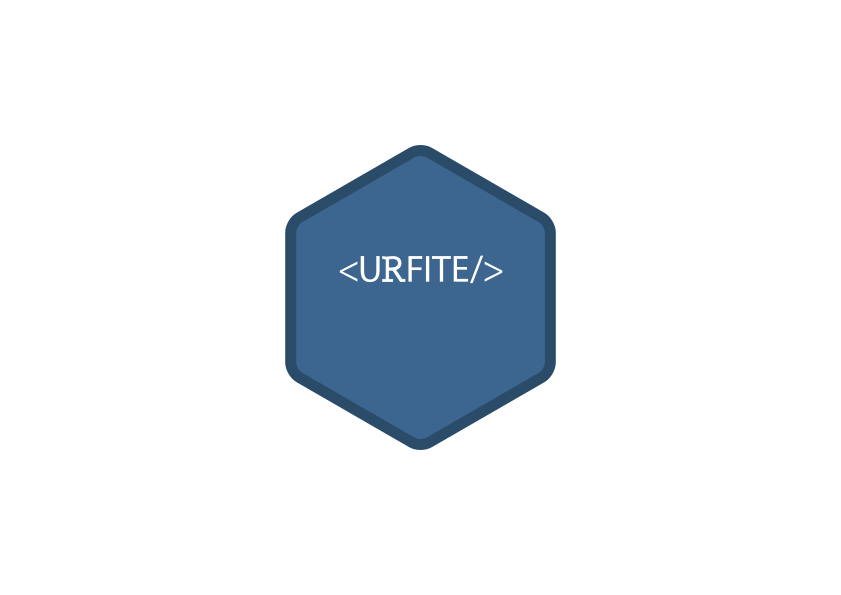
\includegraphics[width=0.45\linewidth]{images/URFITE_logo} \end{center}

\noindent\rule{\textwidth}{1pt}

The interest in the freely available statistical programming language
and software environment \texttt{R} \citep{R-base} is soaring. By the
time we wrote first drafts for this project, more than 11000 addons
(many of them providing cutting-edge methods) were made available on the
Comprehensive \texttt{R} Archive Network
(\href{https://cran.r-project.org/}{CRAN}), an extensive network of FTP
servers around the world that store identical and up-to-date versions of
\texttt{R} code and its documentation. \texttt{R} dominates other
(commercial) software for statistical computing in most fields of
research in applied statistics. The benefits of it being freely
available, open source and having a large and constantly growing
community of users that contribute to CRAN render \texttt{R} more and
more appealing for empirical economists and econometricians alike.

A striking advantage of using \texttt{R} in econometrics is that it
enables students to explicitly document their analysis step-by-step such
that it is easy to update and to expand. This allows to re-use code for
similar applications with different data. Furthermore, \texttt{R}
programs are fully reproducible, which makes it straightforward for
others to comprehend and validate results.

Over the recent years, \texttt{R} has thus become an integral part of
the curricula of econometrics classes we teach at the University of
Duisburg-Essen. In some sense, learning to code is comparable to
learning a foreign language and continuous practice is essential for the
learning success. Needless to say, presenting bare \texttt{R} code on
slides does not encourage the students to engage with hands-on
experience on their own. This is why \texttt{R} is crucial. As for
accompanying literature, there are some excellent books that deal with
\texttt{R} and its applications to econometrics
\citep[e.g.][]{kleiber2008}. However, such sources beyond the scope of
undergraduate students in economics having little understanding of
econometric methods and barely any experience in programming at all.
Consequently, we started to compile a collection of reproducible reports
for use in class. These reports provide guidance on how to implement
selected applications from the textbook \emph{Introduction to
Econometrics} \citep{stock2015} which serves as a basis for the lecture
and the accompanying tutorials. The process is facilitated considerably
by \texttt{knitr} \citep{R-knitr} and \texttt{rmarkdown}
\citep{R-rmarkdown}. In conjunction, both \texttt{R} packages provide
powerful tools for dynamic report generation which allow to seamlessly
combine pure text, LaTeX, \texttt{R} code and its output in a variety of
formats, including PDF and HTML. Being inspired by \emph{Using R for
Introductory Econometrics} \citep{heiss2016}\footnote{\citet{heiss2016}
  builds on the popular \emph{Introductory Econometrics} by
  \citet{wooldridge2016} and demonstrates how to replicate the
  applications discussed therein using \texttt{R}.} and with this
powerful toolkit at hand we wrote up our own empirical companion to
\citet{stock2015}, the result which you to look at, is \textbf{U}sing
\textbf{R} \textbf{f}or \textbf{I}ntroduction \textbf{t}o
\textbf{E}conometrics (\emph{URFITE}).

Similarly to the book by \citet{heiss2016} this project is neither a
comprehensive econometrics textbook nor is it intended to be a general
introduction \texttt{R}. We feel that Stock and Watson do a great job at
explaining the intuition and theory of econometrics, and at any rate
better than we could in yet another introductory textbook! \emph{URFITE}
is best described as an interactive script in the style of a
reproducible research report which aims to provide students with a
platform-independent e-learning arrangement by seamlessly intertwining
theoretical core knowledge and empirical skills in undergraduate
econometrics. Of course, the focus is on empirical applications with
\texttt{R}. We leave out derivations and proofs wherever we can. Our
goal is to enable students not only to learn how results of case studies
can be replicated with \texttt{R} but we also intend to strengthen their
ability in using the newly acquired skills in other empirical
applications --- immediately within \emph{URFITE}.

To realize this, each chapter contains interactive \texttt{R}
programming exercises. These exercises are used as supplements to code
chunks that display how previously discussed techniques can be
implemented within \texttt{R}. They are generated using the
\href{https://github.com/datacamp/datacamp-light}{DataCamp light widget}
and are backed by an \texttt{R} session which is maintained on
\href{https://www.datacamp.com/home}{DataCamp}'s servers. You may play
around with the example exercise presented below.

\begin{center}\textit{This interactive application is only available in the HTML version.}\end{center}

As you can see above, the widget consists of two tabs. \texttt{script.R}
mimics an \texttt{.R}-file, a file format that is commonly used for
storing \texttt{R} code. Lines starting with a \# are commented out,
that is, they are not recognized as code. Furthermore, \texttt{script.R}
works like an exercise sheet where you may write down the solution you
come up with. If you hit the button \emph{Run}, the code will be
executed, submission correctness tests are run and you will be notified
whether your approach is correct. If it is not correct, you will receive
feedback suggesting improvements or hints. The other tab,
\texttt{R Console}, is a fully functional \texttt{R} console that can be
used for trying out solutions to exercises before submitting them. Of
course you may submit (almost any) \texttt{R} code and use the console
to play around and explore. Simply type a command and hit the enter key
on your keyboard.

As an example, consider the following line of code presented in chunk
below. It tells \texttt{R} to compute the number of packages available
on \texttt{CRAN}. The code chunk is followed by the output produced.

\begin{Shaded}
\begin{Highlighting}[]
\CommentTok{# compute the number of packages available on CRAN}
\KeywordTok{nrow}\NormalTok{(}\KeywordTok{available.packages}\NormalTok{(}\DataTypeTok{repos =} \StringTok{"http://cran.us.r-project.org"}\NormalTok{))}
\end{Highlighting}
\end{Shaded}

\begin{verbatim}
## [1] 12740
\end{verbatim}

Each code chunk is equipped with a button on the outer right hand side
which copies the code to your clipboard. This makes it convenient to
work with larger code segments. In the widget above, you may click on
\texttt{R Console} and type \texttt{nrow(available.packages())} (the
command from the code chunk above) and execute it by hitting
\emph{Enter} on your keyboard\footnote{The \texttt{R} session is
  initialized by clicking anywhere into the widget. This might take a
  few seconds. Just wait for the indicator next to the button \emph{Run}
  to turn green.}

Note that some lines in the widget are out-commented which ask you to
assign a numeric value to a variable and then to print the variable's
content to the console. You may enter your solution approach to
\texttt{script.R} and hit the button \emph{Run} in order to get the
feedback described further above. In case you do not know how to solve
this sample exercise (don't panic, that is probably why you are reading
this), a click on \emph{Hint} will provide you with some advice. If you
still can't find a solution, a click on \emph{Solution} will provide you
with another tab, \texttt{Solution.R} which contains sample solution
code. It will often be the case that exercises can be solved in many
different ways and \texttt{Solution.R} presents what we consider as
comprehensible and idiomatic.

\subsubsection*{Conventions Used in this
Book}\label{conventions-used-in-this-book}
\addcontentsline{toc}{subsubsection}{Conventions Used in this Book}

\begin{itemize}
\item
  \emph{Italic} text indicates new terms, names, buttons and alike.
\item
  \texttt{Constant width text}, is generally used in paragraphs to refer
  to \texttt{R} code. This includes commands, variables, functions, data
  types, databases and file names.
\item
  Constant width text on gray background is used to indicate \texttt{R}
  code that can be typed literally by you. It may appear in paragraphs
  for better distinguishability among executable and non-executable code
  statements but it will mostly be encountered in shape of large blocks
  of \texttt{R} code. These blocks are referred to as code chunks (see
  above).
\end{itemize}

\subsubsection*{Acknowledgements}\label{acknowledgements}
\addcontentsline{toc}{subsubsection}{Acknowledgements}

We thank Alexander Blasberg and Kim Hermann for proofreading and their
constructive criticism. We also thank the \emph{Stiferverband für die
Deutsche Wissenschaft e.V.} and the Ministry of Science and Research
North Rhine-Westphalia for their financial support. We are also indebted
to all past students of our introductory econometrics courses at the
University of Duisburg-Essen for their feedback.

\section{\texorpdfstring{A Very Short Introduction to \texttt{R} and
\emph{RStudio}}{A Very Short Introduction to  and RStudio}}\label{a-very-short-introduction-to-and-rstudio}

\begin{figure}[h]

{\centering \includegraphics[width=1\linewidth]{images/rstudio} 

}

\caption{RStudio: the four panes}\label{fig:unnamed-chunk-7}
\end{figure}

\subsubsection*{\texorpdfstring{\texttt{R}
Basics}{ Basics}}\label{basics}
\addcontentsline{toc}{subsubsection}{\texttt{R} Basics}

As mentioned before, this book is not intended to be an introduction to
\texttt{R} but as a guide on how to use its capabilities for
applications commonly encountered in undergraduate econometrics. Those
having basic knowledge in \texttt{R} programming will feel comfortable
starting with Chapter \ref{pt}. This section, however, is meant for
those who have not worked with \texttt{R} or \emph{RStudio} before. If
you at least know how to create objects and call functions, you can skip
it. If you would like to refresh your skills or get a feeling for how to
work with \emph{RStudio}, keep reading.

First of all start \emph{RStudio} and create a new \texttt{R} script by
selecting \emph{File}, \emph{New File}, \emph{R Script}. In the editor
pane, type

\begin{Shaded}
\begin{Highlighting}[]
\DecValTok{1} \OperatorTok{+}\StringTok{ }\DecValTok{1}
\end{Highlighting}
\end{Shaded}

and click on the button labeled \emph{Run} in the top right corner of
the editor. By doing so, your line of code is sent to the console and
the result of this operation should be displayed right underneath it. As
you can see, \texttt{R} works just like a calculator. You can do all
arithmetic calculations by using the corresponding operator (\texttt{+},
\texttt{-}, \texttt{*}, \texttt{/} or \texttt{\textasciicircum{}}). If
you are not sure what the last operator does, try it out and check the
results.

\subsubsection*{Vectors}\label{vectors}
\addcontentsline{toc}{subsubsection}{Vectors}

\texttt{R} is of course more sophisticated than that. We can work with
variables or, more generally, objects. Objects are defined by using the
assignment operator \texttt{<-}. To create a variable named \texttt{x}
which contains the value \texttt{10} type \texttt{x\ \textless{}-\ 10}
and click the button \emph{Run} yet again. The new variable should have
appeared in the environment pane on the top right. The console however
did not show any results, because our line of code did not contain any
call that creates output. When you now type \texttt{x} in the console
and hit return, you ask \texttt{R} to show you the value of \texttt{x}
and the corresponding value should be printed in the console.

\texttt{x} is a scalar, a vector of length \(1\). You can easily create
longer vectors by using the function \texttt{c()} (\emph{c} for
``concatenate'' or ``combine''). To create a vector \texttt{y}
containing the numbers \(1\) to \(5\) and print it, do the following.

\begin{Shaded}
\begin{Highlighting}[]
\NormalTok{y <-}\StringTok{ }\KeywordTok{c}\NormalTok{(}\DecValTok{1}\NormalTok{, }\DecValTok{2}\NormalTok{, }\DecValTok{3}\NormalTok{, }\DecValTok{4}\NormalTok{, }\DecValTok{5}\NormalTok{)}
\NormalTok{y}
\end{Highlighting}
\end{Shaded}

\begin{verbatim}
## [1] 1 2 3 4 5
\end{verbatim}

You can also create a vector of letters or words. For now just remember
that characters have to be surrounded by quotes, else they will be
parsed as object names.

\begin{Shaded}
\begin{Highlighting}[]
\NormalTok{hello <-}\StringTok{ }\KeywordTok{c}\NormalTok{(}\StringTok{"Hello"}\NormalTok{, }\StringTok{"World"}\NormalTok{)}
\end{Highlighting}
\end{Shaded}

Here we have created a vector of length 2 containing the words
\texttt{Hello} and \texttt{World}.

Do not forget to save your script! To do so, select \emph{File},
\emph{Save}.

\subsubsection*{Functions}\label{functions}
\addcontentsline{toc}{subsubsection}{Functions}

You have seen the function \texttt{c()} that can be used to combine
objects. In general, all function calls look the same: a function name
is always followed by round parentheses. Sometimes, the parentheses
include arguments.

Here are two simple examples.

\begin{Shaded}
\begin{Highlighting}[]
\NormalTok{z <-}\StringTok{ }\KeywordTok{seq}\NormalTok{(}\DataTypeTok{from =} \DecValTok{1}\NormalTok{, }\DataTypeTok{to =} \DecValTok{5}\NormalTok{, }\DataTypeTok{by =} \DecValTok{1}\NormalTok{)}

\KeywordTok{mean}\NormalTok{(}\DataTypeTok{x =}\NormalTok{ z)}
\end{Highlighting}
\end{Shaded}

\begin{verbatim}
## [1] 3
\end{verbatim}

In the first line we use a function called \texttt{seq()} to create the
exact same vector as we did in the previous section, calling it
\texttt{z}. The function takes on the arguments \texttt{from},
\texttt{to} and \texttt{by} which should be self-explanatory. The
function \texttt{mean()} computes the arithmetic mean of its argument
\texttt{x}. Since we pass the vector \texttt{z} as the argument
\texttt{x}, the result is \texttt{3}!

If you are not sure which arguments a function expects, you may consult
the function's documentation. Let's say we are not sure how the
arguments required for \texttt{seq()} work. We then type \texttt{?seq}
in the console. By hitting return the documentation page for that
function pops up in the lower right pane of \emph{RStudio}. In there,
the section \emph{Arguments} holds the information we seek. On the
bottom of almost every help page you find examples on how to use the
corresponding functions. This is very helpful for beginners and we
recommend to look out for those.

Of course, all of the commands presented above also work in interactive
widgets throughout the book. You may try them below.

\begin{center}\textit{This interactive application is only available in the HTML version.}\end{center}

\chapter{Probability Theory}\label{pt}

This chapter reviews some basic concepts of probability theory and
demonstrates how they can be applied in \texttt{R}.

Most of the statistical functionalities in \texttt{R}'s standard version
are collected in the \texttt{stats} package. It provides simple
functions which compute descriptive measures and facilitate computations
involving a variety of probability distributions. It also contains more
sophisticated routines that, e.g., enable the user to estimate a large
number of models based on the same data or help to conduct extensive
simulation studies. \texttt{stats} is part of the base distribution of
\texttt{R}, meaning that it is installed by default so there is no need
to run \texttt{install.packages("stats")} or \texttt{library("stats")}.
Simply execute \texttt{library(help\ =\ "stats")} in the console to view
the documentation and a complete list of all functions gathered in
\texttt{stats}. For most packages a documentation that can be viewed
within \emph{RStudio} is available. Documentations can be invoked using
the \texttt{?} operator, e.g., upon execution of \texttt{?stats} the
documentation of the \texttt{stats} package is shown in the help tab of
the bottom-right pane.

In what follows, our focus is on (some of) the probability distributions
that are handled by \texttt{R} and show how to use the relevant
functions to solve simple problems. Thereby, we refresh some core
concepts of probability theory. Among other things, you will learn how
to draw random numbers, how to compute densities, probabilities,
quantiles and alike. As we shall see, it is very convenient to rely on
these routines.

\section{Random Variables and Probability
Distributions}\label{random-variables-and-probability-distributions}

Let us briefly review some basic concepts of probability theory.

\begin{itemize}
\tightlist
\item
  The mutually exclusive results of a random process are called the
  \emph{outcomes}. `Mutually exclusive' means that only one of the
  possible outcomes can be observed.
\item
  We refer to the \emph{probability} of an outcome as the proportion
  that the outcome occurs in the long run, that is, if the experiment is
  repeated very often.
\item
  The set of all possible outcomes of a random variable is called the
  \emph{sample space}.
\item
  An \emph{event} is a subset of the sample space and consists of one or
  more outcomes.
\end{itemize}

These ideas are unified in the concept of a \emph{random variable} which
is a numerical summary of random outcomes. Random variables can be
\emph{discrete} or \emph{continuous}.

\begin{itemize}
\tightlist
\item
  Discrete random variables have discrete outcomes, e.g. \(0\) and
  \(1\).
\item
  A continuous random variable may take on a continuum of possible
  values.
\end{itemize}

\subsection*{Probability Distributions of Discrete Random
Variables}\label{probability-distributions-of-discrete-random-variables}
\addcontentsline{toc}{subsection}{Probability Distributions of Discrete
Random Variables}

A typical example for a discrete random variable \(D\) is the result of
a dice roll: in terms of a random experiment this is nothing but
randomly selecting a sample of size \(1\) from a set of numbers which
are mutually exclusive outcomes. Here, the sample space is
\(\{1,2,3,4,5,6\}\) and we can think of many different events, e.g.,
`the observed outcome lies between \(2\) and \(5\)'.

A basic function to draw random samples from a specified set of elements
is the the function \texttt{sample()}, see \texttt{?sample}. We can use
it to simulate the random outcome of a dice roll. Let's roll the dice!

\begin{Shaded}
\begin{Highlighting}[]
\KeywordTok{sample}\NormalTok{(}\DecValTok{1}\OperatorTok{:}\DecValTok{6}\NormalTok{, }\DecValTok{1}\NormalTok{) }
\end{Highlighting}
\end{Shaded}

\begin{verbatim}
## [1] 4
\end{verbatim}

The probability distribution of a discrete random variable is the list
of all possible values of the variable and their probabilities which sum
to \(1\). The cumulative probability distribution function gives the
probability that the random variable is less than or equal to a
particular value.

For the dice roll, the probability distribution and the cumulative
probability distribution are summarized in Table \ref{tab:pdist}.

\begin{table}

\caption{\label{tab:pdist}PDF and CDF of a Dice Roll}
\centering
\begin{tabular}[t]{l|l|l|l|l|l|l}
\hline
Outcome & 1 & 2 & 3 & 4 & 5 & 6\\
\hline
Probability & 1/6 & 1/6 & 1/6 & 1/6 & 1/6 & 1/6\\
\hline
Cumulative Probability & 1/6 & 2/6 & 3/6 & 4/6 & 5/6 & 1\\
\hline
\end{tabular}
\end{table}

We can easily plot both functions using \texttt{R}. Since the
probability equals \(1/6\) for each outcome, we set up the vector
\texttt{probability} by using the function \texttt{rep()} which
replicates a given value a specified number of times.

\begin{Shaded}
\begin{Highlighting}[]
\CommentTok{# generate the vector of probabilities }
\NormalTok{probability <-}\StringTok{ }\KeywordTok{rep}\NormalTok{(}\DecValTok{1}\OperatorTok{/}\DecValTok{6}\NormalTok{, }\DecValTok{6}\NormalTok{) }

\CommentTok{# plot the probabilites }
\KeywordTok{plot}\NormalTok{(probability, }
     \DataTypeTok{main =} \StringTok{"Probability Distribution"}\NormalTok{,}
     \DataTypeTok{xlab =} \StringTok{"outcomes"}\NormalTok{) }
\end{Highlighting}
\end{Shaded}

\begin{center}\includegraphics{URFITE_files/figure-latex/unnamed-chunk-14-1} \end{center}

For the cumulative probability distribution we need the cumulative
probabilities, i.e., we need the cumulative sums of the vector
\texttt{probability}. These sums can be computed using
\texttt{cumsum()}.

\begin{Shaded}
\begin{Highlighting}[]
\CommentTok{# generate the vector of cumulative probabilities }
\NormalTok{cum_probability <-}\StringTok{ }\KeywordTok{cumsum}\NormalTok{(probability) }

\CommentTok{# plot the probabilites }
\KeywordTok{plot}\NormalTok{(cum_probability, }
     \DataTypeTok{xlab =} \StringTok{"outcomes"}\NormalTok{, }
     \DataTypeTok{main =} \StringTok{"Cumulative Probability Distribution"}\NormalTok{) }
\end{Highlighting}
\end{Shaded}

\begin{center}\includegraphics{URFITE_files/figure-latex/unnamed-chunk-15-1} \end{center}

\subsection*{Bernoulli Trials}\label{bernoulli-trials}
\addcontentsline{toc}{subsection}{Bernoulli Trials}

The set of elements from which \texttt{sample()} draws outcomes does not
have to consist of numbers only. We might as well simulate coin tossing
with outcomes \(H\) (heads) and \(T\) (tails).

\begin{Shaded}
\begin{Highlighting}[]
\KeywordTok{sample}\NormalTok{(}\KeywordTok{c}\NormalTok{(}\StringTok{"H"}\NormalTok{, }\StringTok{"T"}\NormalTok{), }\DecValTok{1}\NormalTok{) }
\end{Highlighting}
\end{Shaded}

\begin{verbatim}
## [1] "H"
\end{verbatim}

The result of a single coin toss is a \emph{Bernoulli} distributed
random variable i.e.~a variable with two possible distinct outcomes.

Imagine you are about to toss a coin \(10\) times in a row and wonder
how likely it is to end up with a \(5\) times heads. This is a typical
example of what we call a \emph{Bernoulli experiment} as it consists of
\(n=10\) Bernoulli trials that are independent of each other and we are
interested in the likelihood of observing \(k=5\) successes \(H\) that
occur with probability \(p=0.5\) (assuming a fair coin) in each trial.
Note that the order of the outcomes does not matter here.

It is a \href{https://en.wikipedia.org/wiki/Binomial_distribution}{well
known result} that the number of successes \(k\) in a Bernoulli
experiment follows a binomial distribution. We denote this as

\[k \sim B(n,p).\]

The probability of observing \(k\) successes in the experiment
\(B(n,p)\) is given by

\[f(k)=P(k)=\begin{pmatrix}n\\ k \end{pmatrix} \cdot p^k \cdot
(1-p)^{n-k}=\frac{n!}{k!(n-k)!} \cdot p^k \cdot (1-p)^{n-k}\]

with \(\begin{pmatrix}n\\ k \end{pmatrix}\) the binomial coefficient.

In \texttt{R}, we can solve the problem stated above by means of the
function \texttt{dbinom()} which calculates the probability of the
binomial distribution given the parameters \texttt{x}, \texttt{size},
and \texttt{prob}, see \texttt{?binom}.

\begin{Shaded}
\begin{Highlighting}[]
\KeywordTok{dbinom}\NormalTok{(}\DataTypeTok{x =} \DecValTok{5}\NormalTok{,}
       \DataTypeTok{size =} \DecValTok{10}\NormalTok{,}
       \DataTypeTok{prob =} \FloatTok{0.5}
\NormalTok{       ) }
\end{Highlighting}
\end{Shaded}

\begin{verbatim}
## [1] 0.2460938
\end{verbatim}

We conclude that the probability of observing Head \(k=5\) times when
tossing the coin \(n=10\) times is about \(24.6\%\).

Now assume we are interested in \(P(4 \leq k \leq 7)\), i.e., the
probability of observing \(4\), \(5\), \(6\) or \(7\) successes for
\(B(10,0.5)\). This may be computed by providing a vector as the
argument \texttt{x} in our call of \texttt{dbinom()} and summing up
using \texttt{sum()}.

\begin{Shaded}
\begin{Highlighting}[]
\CommentTok{# compute P(4 <= k <= 7) using 'dbinom()'}
\KeywordTok{sum}\NormalTok{(}
  \KeywordTok{dbinom}\NormalTok{(}\DataTypeTok{x =} \DecValTok{4}\OperatorTok{:}\DecValTok{7}\NormalTok{, }
         \DataTypeTok{size =} \DecValTok{10}\NormalTok{, }
         \DataTypeTok{prob =} \FloatTok{0.5}\NormalTok{))}
\end{Highlighting}
\end{Shaded}

\begin{verbatim}
## [1] 0.7734375
\end{verbatim}

An alternative approach is to use \texttt{pbinom()}, the distribution
function of the binomial distribution to compute
\[P(4 \leq k \leq 7) = P(k \leq 7) - P(k\leq3 ).\]

\begin{Shaded}
\begin{Highlighting}[]
\CommentTok{# compute P(4 <= k <= 7) using 'pbinom()'}
\KeywordTok{pbinom}\NormalTok{(}\DataTypeTok{size =} \DecValTok{10}\NormalTok{, }\DataTypeTok{prob =} \FloatTok{0.5}\NormalTok{, }\DataTypeTok{q =} \DecValTok{7}\NormalTok{) }\OperatorTok{-}\StringTok{ }\KeywordTok{pbinom}\NormalTok{(}\DataTypeTok{size =} \DecValTok{10}\NormalTok{, }\DataTypeTok{prob =} \FloatTok{0.5}\NormalTok{, }\DataTypeTok{q =} \DecValTok{3}\NormalTok{) }
\end{Highlighting}
\end{Shaded}

\begin{verbatim}
## [1] 0.7734375
\end{verbatim}

The probability distribution of a discrete random variable is nothing
but a list of all possible outcomes that can occur and their respective
probabilities. In the coin tossing example we have \(11\) possible
outcomes for \(k\).

\begin{Shaded}
\begin{Highlighting}[]
\CommentTok{# set up vector of possible outcomes}
\NormalTok{k <-}\StringTok{ }\DecValTok{0}\OperatorTok{:}\DecValTok{10}
\end{Highlighting}
\end{Shaded}

To visualize the probability distribution function of \(k\) we may
therefore do the following:

\begin{Shaded}
\begin{Highlighting}[]
\CommentTok{# assign the probabilities}
\NormalTok{probability <-}\StringTok{ }\KeywordTok{dbinom}\NormalTok{(}\DataTypeTok{x =}\NormalTok{ k,}
                      \DataTypeTok{size =} \DecValTok{10}\NormalTok{, }
                      \DataTypeTok{prob =} \FloatTok{0.5}\NormalTok{)}

\CommentTok{# plot the outcomes against their probabilities}
\KeywordTok{plot}\NormalTok{(}\DataTypeTok{x =}\NormalTok{ k, }
     \DataTypeTok{y =}\NormalTok{ probability,}
     \DataTypeTok{main =} \StringTok{"Probability Distribution Function"}\NormalTok{) }
\end{Highlighting}
\end{Shaded}

\begin{center}\includegraphics{URFITE_files/figure-latex/unnamed-chunk-21-1} \end{center}

In a similar fashion we may plot the cumulative distribution function of
\(k\) by executing the following code chunk:

\begin{Shaded}
\begin{Highlighting}[]
\CommentTok{# compute cumulative probabilities}
\NormalTok{prob <-}\StringTok{ }\KeywordTok{dbinom}\NormalTok{(}\DataTypeTok{x =} \DecValTok{0}\OperatorTok{:}\DecValTok{10}\NormalTok{, }
               \DataTypeTok{size =} \DecValTok{10}\NormalTok{, }
               \DataTypeTok{prob =} \FloatTok{0.5}\NormalTok{)}

\CommentTok{# plot the cumulative probabilities}
\KeywordTok{plot}\NormalTok{(}\DataTypeTok{x =}\NormalTok{ k, }
     \DataTypeTok{y =}\NormalTok{ prob,}
     \DataTypeTok{main =} \StringTok{"Cumulative Distribution Function"}
\NormalTok{     ) }
\end{Highlighting}
\end{Shaded}

\begin{center}\includegraphics{URFITE_files/figure-latex/unnamed-chunk-22-1} \end{center}

\subsection*{Expected Value, Mean and
Variance}\label{expected-value-mean-and-variance}
\addcontentsline{toc}{subsection}{Expected Value, Mean and Variance}

The expected value of a random variable is, loosely, the long-run
average value of its outcomes when the number of repeated trials is
large. For a discrete random variable, the expected value is computed as
a weighted average of its possible outcomes whereby the weights are the
related probabilities. This is formalized in Key Concept 2.1.

\begin{keyconcepts}[Expected Value and the Mean]{2.1}
Suppose the random variable $Y$
takes on $k$ possible values, $y_1, \dots, y_k$, where $y_1$ denotes the first
value, $y_2$ denotes the second value, and so forth, and that the probability
that $Y$ takes on $y_1$ is $p_1$, the probability that $Y$ takes on $y_2$ is
$p_2$ and so forth. The expected value of $Y$, $E(Y)$ is defined as

$$ E(Y) = y_1 p_1 + y_2 p_2 + \cdots + y_k p_k = \sum_{i=1}^k y_i p_i $$

where the notation $\sum_{i=1}^k y_i p_i$ means \"the sum of $y_i$ $p_i$ for $i$
running from $1$ to $k$\". The expected value of $Y$ is also called the mean of $Y$
or the expectation of $Y$ and is denoted by $\mu_Y$.
\end{keyconcepts}

In the dice example, the random variable, \(D\) say, takes on \(6\)
possible values \(d_1 = 1, d_2 = 2, \dots, d_6 = 6\). Assuming a fair
dice, each of the \(6\) outcomes occurs with a probability of \(1/6\).
It is therefore easy to calculate the exact value of \(E(D)\) by hand:

\[ E(D) = 1/6 \sum_{i=1}^6 d_i = 3.5 \]

\(E(D)\) is simply the average of the natural numbers from \(1\) to
\(6\) since all wights \(p_i\) are \(1/6\). This can be easily
calculated using the function \texttt{mean()} which computes the
arithmetic mean of a numeric vector.

\begin{Shaded}
\begin{Highlighting}[]
\CommentTok{# compute mean of natural numbers from 1 to 6}
\KeywordTok{mean}\NormalTok{(}\DecValTok{1}\OperatorTok{:}\DecValTok{6}\NormalTok{)}
\end{Highlighting}
\end{Shaded}

\begin{verbatim}
## [1] 3.5
\end{verbatim}

An example of sampling with replacement is rolling a dice three times in
a row.

\begin{Shaded}
\begin{Highlighting}[]
\CommentTok{# set random seed for reproducibility}
\KeywordTok{set.seed}\NormalTok{(}\DecValTok{1}\NormalTok{)}

\CommentTok{# rolling a dice three times in a row}
\KeywordTok{sample}\NormalTok{(}\DecValTok{1}\OperatorTok{:}\DecValTok{6}\NormalTok{, }\DecValTok{3}\NormalTok{, }\DataTypeTok{replace =}\NormalTok{ T)}
\end{Highlighting}
\end{Shaded}

\begin{verbatim}
## [1] 2 3 4
\end{verbatim}

Of course we could also consider a much bigger number of trials,
\(10000\) say. Doing so, it would be pointless to simply print the
results to the console: by default \texttt{R} displays up to \(1000\)
entries of large vectors and omits the remainder (give it a try).
Eyeballing the numbers does not reveal much. Instead, let us calculate
the sample average of the outcomes using \texttt{mean()} and see if the
result comes close to the expected value \(E(D)=3.5\).

\begin{Shaded}
\begin{Highlighting}[]
\CommentTok{# set random seed for reproducibility}
\KeywordTok{set.seed}\NormalTok{(}\DecValTok{1}\NormalTok{)}

\CommentTok{# compute the sample mean of 10000 dice rolls}
\KeywordTok{mean}\NormalTok{(}\KeywordTok{sample}\NormalTok{(}\DecValTok{1}\OperatorTok{:}\DecValTok{6}\NormalTok{, }
           \DecValTok{10000}\NormalTok{, }
           \DataTypeTok{replace =}\NormalTok{ T))}
\end{Highlighting}
\end{Shaded}

\begin{verbatim}
## [1] 3.5039
\end{verbatim}

We find the sample mean to be fairly close to the expected value. This
result will be discussed in Chapter \ref{RSATDOSA} in more detail.

Other frequently encountered measures are the variance and the standard
deviation. Both are measures of the \emph{dispersion} of a random
variable.

\begin{keyconcepts}[Variance and Standard Deviation]{2.2}
The variance of the discrete \textit{random variable} $Y$, denoted $\sigma^2_Y$, is
$$ \sigma^2_Y = \text{Var}(Y) = E\left[(Y-\mu_Y)^2\right] = \sum_{i=1}^k (y_i - \mu_Y)^2 p_i $$
The standard deviation of $Y$ is $\sigma_Y$, the square root of the variance. The units of the standard deviation are the same as the units of $Y$.
\end{keyconcepts}

The variance as defined in Key Concept 2.2, beeing a population
quantity, \emph{is not} implemented as a function in R. Instead we have
the function \texttt{var()} which computes the \emph{sample variance}

\[ s^2_Y = \frac{1}{n-1} \sum_{i=1}^n (y_i - \overline{y})^2. \]

Remember that \(s^2_Y\) is different from the so called \emph{population
variance} of a discrete random variable \(Y\),

\[ \text{Var}(Y) = \frac{1}{N} \sum_{i=1}^N (y_i - \mu_Y)^2. \]

since it measures how the data is dispersed around the sample average
\(\overline{y}\) instead of the population mean \(\mu_Y\). This becomes
clear when we look at our dice rolling example. For \(D\) we have

\[ \text{Var}(D) = 1/6 \sum_{i=1}^6 (d_i - 3.5)^2 = 2.92  \] which is
obviously different from the result of \(s^2\) as computed by
\texttt{var()}.

\begin{Shaded}
\begin{Highlighting}[]
\KeywordTok{var}\NormalTok{(}\DecValTok{1}\OperatorTok{:}\DecValTok{6}\NormalTok{)}
\end{Highlighting}
\end{Shaded}

\begin{verbatim}
## [1] 3.5
\end{verbatim}

The sample variance as computed by \texttt{var()} is an \emph{estimator}
of the population variance.

 \# You may use this widget to play around with the functions presented
above

\subsection*{Probability Distributions of Continuous Random
Variables}\label{probability-distributions-of-continuous-random-variables}
\addcontentsline{toc}{subsection}{Probability Distributions of
Continuous Random Variables}

Since a continuous random variable takes on a continuum of possible
values, we cannot use the concept of a probability distribution as used
for discrete random variables. Instead, the probability distribution of
a continuous random variable is summarized by its \emph{probability
density function} (PDF).

The cumulative probability distribution function (CDF) for a continuous
random variable is defined just as in the discrete case. Hence, the
cumulative probability distribution of a continuous random variables
states the probability that the random variable is less than or equal to
a particular value.

For completeness, we present revisions of Key Concepts 2.1 and 2.2 for
the continuous case.

\begin{keyconcepts}[Probabilities\comma Expected Value and Variance of a Continuous Random Variable]{2.3}
Let $f_Y(y)$ denote the probability density function of $Y$. The Probability that $Y$ falls between $a$ and $b$ where $a < b$ is 
$$ P(a \leq Y \leq b) = \int_a^b f_Y(y) \mathrm{d}y. $$
We further have that $P(-\infty \leq Y \leq \infty) = 1$ and therefore $\int_{-\infty}^{\infty} f_Y(y) \mathrm{d}y = 1$.

As for the discrete case, the expected value of $Y$ is the probability weighted average of its values. Due to continuity, we use integrals instead of sums. The expected value of $Y$ is defined as

$$ E(Y) =  \mu_Y = \int y f_Y(y) \mathrm{d}y. $$

The variance is the expected value of $(Y - \mu_Y)^2$. We thus have

$$\text{Var}(Y) =  \sigma_Y^2 = \int (y - \mu_Y)^2 f_Y(y) \mathrm{d}y.$$
\end{keyconcepts}

Let us discuss an example:

Consider the continuous random variable \(X\) with probability density
function

\[ f_X(x) = \frac{3}{x^4}, x>1. \]

\begin{itemize}
\tightlist
\item
  We can show analytically that the integral of \(f_X(x)\) over the real
  line equals \(1\).
\end{itemize}

\begin{align}
 \int f_X(x) \mathrm{d}x =&  \int_{1}^{\infty} \frac{3}{x^4} \mathrm{d}x \\
  =& \lim_{t \rightarrow \infty} \int_{1}^{t} \frac{3}{x^4} \mathrm{d}x \\
  =& \lim_{t \rightarrow \infty}  -x^{-3} \rvert_{x=1}^t \\
  =& -\left(\lim_{t \rightarrow \infty}\frac{1}{t^3} - 1\right) \\
  =& 1
\end{align}

\begin{itemize}
\tightlist
\item
  The expectation of \(X\) can be computed as follows:
\end{itemize}

\begin{align}
 E(X) = \int x \cdot f_X(x) \mathrm{d}x =&  \int_{1}^{\infty} x \cdot \frac{3}{x^4} \mathrm{d}x \\
  =& - \frac{3}{2} x^{-2} \rvert_{x=1}^{\infty} \\
  =& -\frac{3}{2} \left( \lim_{t \rightarrow \infty} \frac{1}{t^2} - 1 \right) \\
  =& \frac{3}{2}
\end{align}

\begin{itemize}
\tightlist
\item
  Note that the variance of \(X\) can be expressed as
  \(\text{Var}(X) = E(X^2) - E(X)^2\). Since \(E(X)\) has been computed
  in the previous step, we seek \(E(X^2)\):
\end{itemize}

\begin{align}
 E(X^2)= \int x^2 \cdot f_X(x) \mathrm{d}x =&  \int_{1}^{\infty} x^2 \cdot \frac{3}{x^4} \mathrm{d}x \\
  =& -3 x^{-1} \rvert_{x=1}^{\infty} \\
  =& -3 \left( \lim_{t \rightarrow \infty} \frac{1}{t} - 1 \right) \\
  =& 3
\end{align}

So we have shown that the area under the curve equals one, that the
expectation is \(E(X)=\frac{3}{2} \ \) and we found the variance to be
\(\text{Var}(X) = \frac{3}{4}\). However, this was tedious and, as we
shall see, an analytic approach is not applicable for some probability
density functions, e.g., if integrals have no closed form solutions.

Luckily, \texttt{R} also enables us to easily find the results derived
above. The tool we use for this is the function \texttt{integrate()}.
First, we have to define the functions we want to calculate integrals
for as \texttt{R} functions, i.e., the PDF \(f_X(x)\) as well as the
expressions \(x\cdot f_X(x)\) and \(x^2\cdot f_X(x)\).

\begin{Shaded}
\begin{Highlighting}[]
\CommentTok{# define functions}
\NormalTok{f <-}\StringTok{ }\ControlFlowTok{function}\NormalTok{(x) }\DecValTok{3}\OperatorTok{/}\NormalTok{x}\OperatorTok{^}\DecValTok{4}
\NormalTok{g <-}\StringTok{ }\ControlFlowTok{function}\NormalTok{(x) x}\OperatorTok{*}\KeywordTok{f}\NormalTok{(x)}
\NormalTok{h <-}\StringTok{ }\ControlFlowTok{function}\NormalTok{(x) x}\OperatorTok{^}\DecValTok{2}\OperatorTok{*}\KeywordTok{f}\NormalTok{(x)}
\end{Highlighting}
\end{Shaded}

Next, we use \texttt{integrate()} and set lower and upper limits of
integration to \(1\) and \(\infty\) using arguments \texttt{lower} and
\texttt{upper}. By default, \texttt{integrate()} prints the result along
with an estimate of the approximation error to the console. However, the
outcome is not a numeric value one can readily do further calculation
with. In order to get only a numeric value of the integral, we need to
use the \texttt{\$} operator in conjunction with \texttt{value}. The
\texttt{\$} operator is used to extract elements by name from an object
of type \texttt{list}.

\begin{Shaded}
\begin{Highlighting}[]
\CommentTok{# compute area under the density curve}
\NormalTok{area <-}\StringTok{ }\KeywordTok{integrate}\NormalTok{(f, }
                 \DataTypeTok{lower =} \DecValTok{1}\NormalTok{, }
                 \DataTypeTok{upper =} \OtherTok{Inf}\NormalTok{)}\OperatorTok{$}\NormalTok{value}
\NormalTok{area }
\end{Highlighting}
\end{Shaded}

\begin{verbatim}
## [1] 1
\end{verbatim}

\begin{Shaded}
\begin{Highlighting}[]
\CommentTok{# compute E(X)}
\NormalTok{EX <-}\StringTok{ }\KeywordTok{integrate}\NormalTok{(g,}
                \DataTypeTok{lower =} \DecValTok{1}\NormalTok{,}
                \DataTypeTok{upper =} \OtherTok{Inf}\NormalTok{)}\OperatorTok{$}\NormalTok{value}
\NormalTok{EX}
\end{Highlighting}
\end{Shaded}

\begin{verbatim}
## [1] 1.5
\end{verbatim}

\begin{Shaded}
\begin{Highlighting}[]
\CommentTok{# compute Var(X)}
\NormalTok{VarX <-}\StringTok{ }\KeywordTok{integrate}\NormalTok{(h,}
                  \DataTypeTok{lower =} \DecValTok{1}\NormalTok{,}
                  \DataTypeTok{upper =} \OtherTok{Inf}
\NormalTok{                  )}\OperatorTok{$}\NormalTok{value }\OperatorTok{-}\StringTok{ }\NormalTok{EX}\OperatorTok{^}\DecValTok{2} 
\NormalTok{VarX}
\end{Highlighting}
\end{Shaded}

\begin{verbatim}
## [1] 0.75
\end{verbatim}

Although there is a wide variety of distributions, the ones most often
encountered in econometrics are the normal, chi-squared, Student \(t\)
and \(F\) distributions. Therefore we will discuss some core \texttt{R}
functions that allow to do calculations involving densities,
probabilities and quantiles of these distributions.

Every probability distribution that \texttt{R} handles has four basic
functions whose names consist of a prefix followed by a root name. As an
example, take the normal distribution. The root name of all four
functions associated with the normal distribution is \texttt{norm}. The
four prefixes are

\begin{itemize}
\tightlist
\item
  \texttt{d} for ``density'' - probability function / probability
  density function
\item
  \texttt{p} for ``probability'' - cumulative distribution function
\item
  \texttt{q} for ``quantile'' - quantile function (inverse cumulative
  distribution function)
\item
  \texttt{r} for ``random'' - random number generator
\end{itemize}

Thus, for the normal distribution we have the \texttt{R} functions
\texttt{dnorm()}, \texttt{pnorm()}, \texttt{qnorm()} and
\texttt{rnorm()}.

\subsection*{The Normal Distribution}\label{the-normal-distribution}
\addcontentsline{toc}{subsection}{The Normal Distribution}

The probably most important probability distribution considered here is
the normal distribution. This is not least due to the special role of
the standard normal distribution and the Central Limit Theorem which is
to be treated shortly. Normal distributions are symmetric and
bell-shaped. A normal distribution is characterized by its mean \(\mu\)
and its standard deviation \(\sigma\), concisely expressed by
\(N(\mu,\sigma^2)\). The normal distribution has the PDF

\begin{align}
f(x) = \frac{1}{\sqrt{2 \pi} \sigma} \exp{-(x - μ)^2/(2 σ^2)}.
\end{align}

For the standard normal distribution we have \(\mu=0\) and \(\sigma=1\).
Standard normal variates are often denoted by \(Z\). Usually, the
standard normal PDF is denoted by \(\phi\) and the standard normal CDF
is denoted by \(\Phi\). Hence,
\[ \phi(c) = \Phi'(c) \ \ , \ \ \Phi(c) = P(Z \leq c) \ \ , \ \ Z \sim N(0,1).\]
In \texttt{R}, we can conveniently obtain density values of normal
distributions using the function \texttt{dnorm()}. Let us draw a plot of
the standard normal density function using \texttt{curve()} in
conjunction with \texttt{dnorm()}.

\begin{Shaded}
\begin{Highlighting}[]
\CommentTok{# draw a plot of the N(0,1) PDF}
\KeywordTok{curve}\NormalTok{(}\KeywordTok{dnorm}\NormalTok{(x),}
      \DataTypeTok{xlim=}\KeywordTok{c}\NormalTok{(}\OperatorTok{-}\FloatTok{3.5}\NormalTok{, }\FloatTok{3.5}\NormalTok{),}
      \DataTypeTok{ylab =} \StringTok{"Density"}\NormalTok{, }
      \DataTypeTok{main =} \StringTok{"Standard Normal Density Function"}
\NormalTok{      ) }
\end{Highlighting}
\end{Shaded}

\begin{center}\includegraphics{URFITE_files/figure-latex/unnamed-chunk-35-1} \end{center}

We can obtain the density at different positions by passing a vector of
quantiles to \texttt{dnorm()}.

\begin{Shaded}
\begin{Highlighting}[]
\CommentTok{# compute denstiy at x=-1.96, x=0 and x=1.96}
\KeywordTok{dnorm}\NormalTok{(}\DataTypeTok{x =} \KeywordTok{c}\NormalTok{(}\OperatorTok{-}\FloatTok{1.96}\NormalTok{, }\DecValTok{0}\NormalTok{, }\FloatTok{1.96}\NormalTok{))}
\end{Highlighting}
\end{Shaded}

\begin{verbatim}
## [1] 0.05844094 0.39894228 0.05844094
\end{verbatim}

Similar to the PDF, we can plot the standard normal CDF using
\texttt{curve()} and \texttt{pnorm()}.

\begin{Shaded}
\begin{Highlighting}[]
\CommentTok{# plot the standard normal CDF}
\KeywordTok{curve}\NormalTok{(}\KeywordTok{pnorm}\NormalTok{(x), }
      \DataTypeTok{xlim=}\KeywordTok{c}\NormalTok{(}\OperatorTok{-}\FloatTok{3.5}\NormalTok{, }\FloatTok{3.5}\NormalTok{), }
      \DataTypeTok{ylab =} \StringTok{"Density"}\NormalTok{, }
      \DataTypeTok{main =} \StringTok{"Standard Normal Cumulative Distribution Function"}
\NormalTok{      )}
\end{Highlighting}
\end{Shaded}

\begin{center}\includegraphics{URFITE_files/figure-latex/unnamed-chunk-37-1} \end{center}

We can also use \texttt{R} to calculate the probability of events
associated with a standard normal variate.

Let us say we are interested in \(P(Z \leq 1,337)\). For some continuous
random variable \(Z\) on \([-\infty,\infty]\) with density function
\(g(x)\) we would have to determine \(G(x)\) which is the anti
derivative of \(g(x)\) so that

\[ P(Z \leq 1,337 ) = G(1,337) = \int_{-\infty}^{1,337} g(x) \mathrm{d}x.  \]

If \(Z \sim N(0,1)\), we have \(g(x)=\phi(x)\). There is no analytic
solution to the integral above and it is cumbersome to come up with an
approximation. However, we may circumvent this using \texttt{R} in
different ways. The first approach makes use of the function
\texttt{integrate()} which allows to solve one-dimensional integration
problems using a numerical method. For this, we first define the
function we want to compute the integral of as a \texttt{R} function
\texttt{f}. In our example, \texttt{f} needs to be the standard normal
density function and hence takes a single argument \texttt{x}. Following
the definition of \(\phi(x)\) we define \texttt{f} as

\begin{Shaded}
\begin{Highlighting}[]
\CommentTok{# define the standard normal PDF as a R function}
\NormalTok{f <-}\StringTok{ }\ControlFlowTok{function}\NormalTok{(x) \{}
  \DecValTok{1}\OperatorTok{/}\NormalTok{(}\KeywordTok{sqrt}\NormalTok{(}\DecValTok{2} \OperatorTok{*}\StringTok{ }\NormalTok{pi)) }\OperatorTok{*}\StringTok{ }\KeywordTok{exp}\NormalTok{(}\OperatorTok{-}\FloatTok{0.5} \OperatorTok{*}\StringTok{ }\NormalTok{x}\OperatorTok{^}\DecValTok{2}\NormalTok{)}
\NormalTok{\}}
\end{Highlighting}
\end{Shaded}

Let us check if this function enables us to compute standard normal
density values by passing it a vector of quantiles.

\begin{Shaded}
\begin{Highlighting}[]
\CommentTok{# define vector of quantiles}
\NormalTok{quants <-}\StringTok{ }\KeywordTok{c}\NormalTok{(}\OperatorTok{-}\FloatTok{1.96}\NormalTok{, }\DecValTok{0}\NormalTok{, }\FloatTok{1.96}\NormalTok{)}

\CommentTok{# compute density values}
\KeywordTok{f}\NormalTok{(quants)}
\end{Highlighting}
\end{Shaded}

\begin{verbatim}
## [1] 0.05844094 0.39894228 0.05844094
\end{verbatim}

\begin{Shaded}
\begin{Highlighting}[]
\CommentTok{# compare to results produced by dnorm()}
\KeywordTok{f}\NormalTok{(quants) }\OperatorTok{==}\StringTok{ }\KeywordTok{dnorm}\NormalTok{(quants)}
\end{Highlighting}
\end{Shaded}

\begin{verbatim}
## [1] TRUE TRUE TRUE
\end{verbatim}

Notice that the results produced by \texttt{f()} are indeed equivalent
to those given by \texttt{dnorm()}.

Next, we call \texttt{integrate()} on \texttt{f()} and specify the
arguments \texttt{lower} and \texttt{upper}, the lower and upper limits
of integration.

\begin{Shaded}
\begin{Highlighting}[]
\CommentTok{# integrate f()}
\KeywordTok{integrate}\NormalTok{(f, }
          \DataTypeTok{lower =} \OperatorTok{-}\OtherTok{Inf}\NormalTok{, }
          \DataTypeTok{upper =} \FloatTok{1.337}
\NormalTok{          )}
\end{Highlighting}
\end{Shaded}

\begin{verbatim}
## 0.9093887 with absolute error < 1.7e-07
\end{verbatim}

We find that the probability of observing \(Z \leq 1.337\) is about
\(0.9094\%\).

A second and much more convenient way is to use the function
\texttt{pnorm()} which also allows calculus involving the standard
normal cumulative distribution function.

\begin{Shaded}
\begin{Highlighting}[]
\CommentTok{# compute the probability using pnorm()}
\KeywordTok{pnorm}\NormalTok{(}\FloatTok{1.337}\NormalTok{)}
\end{Highlighting}
\end{Shaded}

\begin{verbatim}
## [1] 0.9093887
\end{verbatim}

The result matches the outcome of the approach using
\texttt{integrate()}.

Let us discuss some further examples:

A commonly known result is that \(95\%\) probability mass of a standard
normal lies in the interval \([-1.96, 1.96]\), that is in a distance of
about \(2\) standard deviations to the mean. We can easily confirm this
by calculating

\[ P(-1.96 \leq Z \leq 1.96) = 1-2\times P(Z \leq -1.96) \] due to
symmetry of the standard normal PDF. Thanks to \texttt{R}, we can
abandon the table of the standard normal CDF again and instead solve
this by using the function \texttt{pnorm()}.

\begin{Shaded}
\begin{Highlighting}[]
\CommentTok{# compute the probability}
\DecValTok{1} \OperatorTok{-}\StringTok{ }\DecValTok{2} \OperatorTok{*}\StringTok{ }\NormalTok{(}\KeywordTok{pnorm}\NormalTok{(}\OperatorTok{-}\FloatTok{1.96}\NormalTok{)) }
\end{Highlighting}
\end{Shaded}

\begin{verbatim}
## [1] 0.9500042
\end{verbatim}

Now consider a random variable \(Y\) with \(Y \sim N(5, 25)\). To make
statements about the probability of observing outcomes of \(Y\) in some
specific range is more convenient without when we standardize first as
shown in Key Concept 2.4.

\begin{keyconcepts}[Computing Probabilities Involving Normal Random Variables]{2.4}

Suppose $Y$ is normally distributed with mean $\mu$ and variance $\sigma^2$: $$Y
\sim N(\mu, \sigma^2)$$ Then $Y$ is standardized by subtracting its mean and
dividing by its standard deviation: $$ Z = \frac{Y -\mu}{\sigma} $$ Let $c_1$
and $c_2$ denote two numbers whereby $c_1 < c_2$ and further $d_1 = (c_1 - \mu)
/ \sigma$ and $d_2 = (c_2 - \mu)/\sigma$. Then
\begin{align*} 
P(Y \leq c_2) =& \, P(Z \leq d_2) = \Phi(d_2) \\ 
P(Y \geq c_1) =& \, P(Z \geq d_1) = 1 - \Phi(d_1) \\ 
P(c_1 \leq Y \leq c_2) =& \, P(d_1 \leq Z \leq d_2) = \Phi(d_2) - \Phi(d_1). 
\end{align*}
\end{keyconcepts}

\texttt{R} functions that handle the normal distribution can perform
this standardization. If we are interested in \(P(3 \leq Y \leq 4)\) we
can use \texttt{pnorm()} and adjust for a mean and/or a standard
deviation that deviate from \(\mu=0\) and \(\sigma = 1\) by specifying
the arguments \texttt{mean} and \texttt{sd} accordingly.
\textbf{Attention}: the argument \texttt{sd} requires the standard
deviation, not the variance!

\begin{Shaded}
\begin{Highlighting}[]
\KeywordTok{pnorm}\NormalTok{(}\DecValTok{4}\NormalTok{, }\DataTypeTok{mean =} \DecValTok{5}\NormalTok{, }\DataTypeTok{sd =} \DecValTok{5}\NormalTok{) }\OperatorTok{-}\StringTok{ }\KeywordTok{pnorm}\NormalTok{(}\DecValTok{3}\NormalTok{, }\DataTypeTok{mean =} \DecValTok{5}\NormalTok{, }\DataTypeTok{sd =} \DecValTok{5}\NormalTok{) }
\end{Highlighting}
\end{Shaded}

\begin{verbatim}
## [1] 0.07616203
\end{verbatim}

An extension of the normal distribution in a univariate setting is the
multivariate normal distribution. The PDF of two random normal variables
\(X\) and \(Y\) is given by

\begin{align}
\begin{split}
g_{X,Y}(x,y) =& \, \frac{1}{2\pi\sigma_X\sigma_Y\sqrt{1-\rho_{XY}^2}} \\ 
\cdot & \, \exp \left\{ \frac{1}{-2(1-\rho_{XY}^2)} \left[ \left( \frac{x-\mu_x}{\sigma_x} \right)^2 - 2\rho_{XY}\left( \frac{x-\mu_X}{\sigma_X} \right)\left( \frac{y-\mu_Y}{\sigma_Y} \right) + \left( \frac{y-\mu_Y}{\sigma_Y} \right)^2 \right]  \right\}.
\end{split} \label{eq:bivnorm}
\end{align}

Equation \eqref{eq:bivnorm} contains the bivariate normal PDF. Admittedly,
it is hard to gain insights from this complicated expression. Instead,
let us consider the special case where \(X\) and \(Y\) are uncorrelated
standard normal random variables with density functions \(f_X(x)\) and
\(f_Y(y)\) and we assume that they have a joint normal distribution. We
then have the parameters \(\sigma_X = \sigma_Y = 1\), \(\mu_X=\mu_Y=0\)
(due to marginal standard normality) and \(\rho_{XY}=0\) (due to
independence). The joint probability density function of \(X\) and \(Y\)
then becomes

\[ g_{X,Y}(x,y) = f_X(x) f_Y(y) = \frac{1}{2\pi} \cdot \exp \left\{ -\frac{1}{2} \left[x^2 + y^2 \right]  \right\}, \tag{2.2}  \]

the PDF of the bivariate standard normal distribution. The next plot
provides an interactive three-dimensional plot of (2.2). By moving the
cursor over the plot you can see that the density is rotationally
invariant.

\subsection*{The Chi-Squared
Distribution}\label{the-chi-squared-distribution}
\addcontentsline{toc}{subsection}{The Chi-Squared Distribution}

Another distribution relevant in econometric day-to-day work is the
chi-squared distribution. It is often needed when testing special types
of hypotheses frequently encountered when dealing with regression
models.

The sum of \(M\) squared independent standard normal distributed random
variables follows a chi-squared distribution with \(M\) degrees of
freedom.

\[ Z_1^2 + \dots + Z_M^2 = \sum_{m=1}^M Z_m^2 \sim \chi^2_M \ \ \text{with} \ \ Z_m \overset{i.i.d.}{\sim} N(0,1) \label{eq:chisq}\]

A \(\chi^2\) distributed random variable with \(M\) degrees of freedom
has expectation \(M\), mode at \(M-2\) for \(n \geq 2\) and variance
\(2 \cdot M\).

For example, if we have

\[ Z_1,Z_2,Z_3 \overset{i.i.d.}{\sim} N(0,1) \]

it holds that

\[ Z_1^2+Z_2^2+Z_3^3 \sim \chi^2_3. \tag{2.3} \] Using the code below,
we can display the PDF and the CDF of a \(\chi^2_3\) random variable in
a single plot. This is achieved by setting the argument
\texttt{add = TRUE} in the second call of \texttt{curve()}. Further we
adjust limits of both axes using \texttt{xlim} and \texttt{ylim} and
choose different colors to make both functions better distinguishable.
The plot is completed by adding a legend with help of the function
\texttt{legend()}.

\begin{Shaded}
\begin{Highlighting}[]
\CommentTok{# plot the PDF}
\KeywordTok{curve}\NormalTok{(}\KeywordTok{dchisq}\NormalTok{(x, }\DataTypeTok{df=}\DecValTok{3}\NormalTok{), }
      \DataTypeTok{xlim =} \KeywordTok{c}\NormalTok{(}\DecValTok{0}\NormalTok{, }\DecValTok{10}\NormalTok{), }
      \DataTypeTok{ylim =} \KeywordTok{c}\NormalTok{(}\DecValTok{0}\NormalTok{, }\DecValTok{1}\NormalTok{), }
      \DataTypeTok{col =} \StringTok{"blue"}\NormalTok{,}
      \DataTypeTok{ylab =} \StringTok{""}\NormalTok{,}
      \DataTypeTok{main =} \StringTok{"p.d.f. and c.d.f of Chi-Squared Distribution, M = 3"}
\NormalTok{      )}

\CommentTok{# add the CDF to the plot}
\KeywordTok{curve}\NormalTok{(}\KeywordTok{pchisq}\NormalTok{(x, }\DataTypeTok{df =} \DecValTok{3}\NormalTok{), }
      \DataTypeTok{xlim=}\KeywordTok{c}\NormalTok{(}\DecValTok{0}\NormalTok{, }\DecValTok{10}\NormalTok{), }
      \DataTypeTok{add =} \OtherTok{TRUE}\NormalTok{, }
      \DataTypeTok{col =} \StringTok{"red"}
\NormalTok{      )}

\CommentTok{# add a legend to the plot}
\KeywordTok{legend}\NormalTok{(}\StringTok{"topleft"}\NormalTok{, }
       \KeywordTok{c}\NormalTok{(}\StringTok{"PDF"}\NormalTok{, }\StringTok{"CDF"}\NormalTok{), }
       \DataTypeTok{col =} \KeywordTok{c}\NormalTok{(}\StringTok{"blue"}\NormalTok{, }\StringTok{"red"}\NormalTok{), }
       \DataTypeTok{lty =} \KeywordTok{c}\NormalTok{(}\DecValTok{1}\NormalTok{, }\DecValTok{1}\NormalTok{)}
\NormalTok{       )}
\end{Highlighting}
\end{Shaded}

\begin{center}\includegraphics{URFITE_files/figure-latex/unnamed-chunk-47-1} \end{center}

Since the outcomes of a \(\chi^2_M\) distributed random variable are
always positive, the domain of the related PDF and CDF is
\(\mathbb{R}_{\geq0}\).

As expectation and variance depend (solely!) on the degrees of freedom,
the distribution's shape changes drastically if we vary the number of
squared standard normals that are summed up. This relation is often
depicted by overlaying densities for different \(M\), see e.g.~the
Wikipedia Article.

Start by plotting the density of the \(\chi_1^2\) distribution on the
interval \([0,15]\) with \texttt{curve()}. In the next step, we loop
over degrees of freedom \(m=2,...,7\) and add a density curve for each
\(m\) to the plot. We also adjust the line color for each iteration of
the loop by setting \texttt{col = m}. At last, we add a legend that
displays degrees of freedom and the associated colors.

\begin{Shaded}
\begin{Highlighting}[]
\CommentTok{# plot the density for m=1}
\KeywordTok{curve}\NormalTok{(}\KeywordTok{dchisq}\NormalTok{(x, }\DataTypeTok{df =} \DecValTok{1}\NormalTok{), }
      \DataTypeTok{xlim =} \KeywordTok{c}\NormalTok{(}\DecValTok{0}\NormalTok{, }\DecValTok{15}\NormalTok{), }
      \DataTypeTok{xlab =} \StringTok{"x"}\NormalTok{, }
      \DataTypeTok{ylab =} \StringTok{"Density"}\NormalTok{, }
      \DataTypeTok{main =} \StringTok{"Chi-Square Distributed Random Variables"}
\NormalTok{      )}

\CommentTok{# add densities for m=2,...,7 to the plot using a 'for' loop }
\ControlFlowTok{for}\NormalTok{ (m }\ControlFlowTok{in} \DecValTok{2}\OperatorTok{:}\DecValTok{7}\NormalTok{) \{}
  \KeywordTok{curve}\NormalTok{(}\KeywordTok{dchisq}\NormalTok{(x, }\DataTypeTok{df =}\NormalTok{ m),}
        \DataTypeTok{xlim =} \KeywordTok{c}\NormalTok{(}\DecValTok{0}\NormalTok{, }\DecValTok{15}\NormalTok{), }
        \DataTypeTok{add =}\NormalTok{ T, }
        \DataTypeTok{col =}\NormalTok{ m}
\NormalTok{        )}
\NormalTok{\}}

\CommentTok{# add a legend}
\KeywordTok{legend}\NormalTok{(}\StringTok{"topright"}\NormalTok{, }
       \KeywordTok{as.character}\NormalTok{(}\DecValTok{1}\OperatorTok{:}\DecValTok{7}\NormalTok{), }
       \DataTypeTok{col =} \DecValTok{1}\OperatorTok{:}\DecValTok{7}\NormalTok{ , }
       \DataTypeTok{lty =} \DecValTok{1}\NormalTok{, }
       \DataTypeTok{title =} \StringTok{"D.f."}
\NormalTok{       )}
\end{Highlighting}
\end{Shaded}

\begin{center}\includegraphics{URFITE_files/figure-latex/unnamed-chunk-48-1} \end{center}

It is evident that increasing the degrees of freedom shifts the
distribution to the right (the mode becomes larger) and increases the
dispersion (the distribution's variance grows).

\subsection*{The Student t Distribution}\label{thetdist}
\addcontentsline{toc}{subsection}{The Student t Distribution}

Let \(Z\) be a standard normal variate, \(W\) a random variable that
follows a \(\chi^2_M\) distribution with \(M\) degrees of freedom and
further assume that \(Z\) and \(W\) are independently distributed. Then
it holds that

\[ \frac{Z}{\sqrt{W/M}} =:X \sim t_M \] and \(X\) follows a
\emph{Student \(t\) distribution} (or simply \(t\) distribution) with
\(M\) degrees of freedom.

Similar to the \(\chi^2_M\) distribution, the shape of a \(t_M\)
distribution depends on \(M\). \(t\) distributions are symmetric,
bell-shaped and look very similar to a normal distribution, especially
when \(M\) is large. This is not a coincidence: for a sufficient large
\(M\), the \(t_M\) distribution can be approximated by the standard
normal distribution. This approximation works reasonably well for
\(M\geq 30\). As we will show later by means of a small simulation
study, the \(t_{\infty}\) distribution \emph{is} the standard normal
distribution.

A \(t_M\) distributed random variable has an expectation if \(M>1\) and
it has a variance if \(M>2\).

\begin{align}
  E(X) =& 0 \ , \ M>1 \\
  \text{Var}(X) =& \frac{M}{M-2} \ , \ M>2
\end{align}

Let us graph some \(t\) distributions with different \(M\) and compare
them to the standard normal distribution.

\begin{Shaded}
\begin{Highlighting}[]
\CommentTok{# plot the standard normal density}
\KeywordTok{curve}\NormalTok{(}\KeywordTok{dnorm}\NormalTok{(x), }
      \DataTypeTok{xlim =} \KeywordTok{c}\NormalTok{(}\OperatorTok{-}\DecValTok{4}\NormalTok{,}\DecValTok{4}\NormalTok{), }
      \DataTypeTok{xlab =} \StringTok{"x"}\NormalTok{, }
      \DataTypeTok{lty =} \DecValTok{2}\NormalTok{, }
      \DataTypeTok{ylab =} \StringTok{"Density"}\NormalTok{, }
      \DataTypeTok{main =} \StringTok{"Theoretical Densities of t Distributions"}
\NormalTok{      )}

\CommentTok{# plot the t density for m=2}
\KeywordTok{curve}\NormalTok{(}\KeywordTok{dt}\NormalTok{(x, }\DataTypeTok{df =} \DecValTok{2}\NormalTok{), }
      \DataTypeTok{xlim =} \KeywordTok{c}\NormalTok{(}\OperatorTok{-}\DecValTok{4}\NormalTok{, }\DecValTok{4}\NormalTok{), }
      \DataTypeTok{col =} \DecValTok{2}\NormalTok{, }
      \DataTypeTok{add =}\NormalTok{ T}
\NormalTok{      )}

\CommentTok{# plot the t density for m=4}
\KeywordTok{curve}\NormalTok{(}\KeywordTok{dt}\NormalTok{(x, }\DataTypeTok{df =} \DecValTok{4}\NormalTok{), }
      \DataTypeTok{xlim =} \KeywordTok{c}\NormalTok{(}\OperatorTok{-}\DecValTok{4}\NormalTok{, }\DecValTok{4}\NormalTok{), }
      \DataTypeTok{col =} \DecValTok{3}\NormalTok{, }
      \DataTypeTok{add =}\NormalTok{ T}
\NormalTok{      )}

\CommentTok{# plot the t density for m=25}
\KeywordTok{curve}\NormalTok{(}\KeywordTok{dt}\NormalTok{(x, }\DataTypeTok{df =} \DecValTok{25}\NormalTok{), }
      \DataTypeTok{xlim =} \KeywordTok{c}\NormalTok{(}\OperatorTok{-}\DecValTok{4}\NormalTok{, }\DecValTok{4}\NormalTok{), }
      \DataTypeTok{col =} \DecValTok{4}\NormalTok{, }
      \DataTypeTok{add =}\NormalTok{ T}
\NormalTok{      )}

\CommentTok{# add a legend}
\KeywordTok{legend}\NormalTok{(}\StringTok{"topright"}\NormalTok{, }
       \KeywordTok{c}\NormalTok{(}\StringTok{"N(0,1)"}\NormalTok{,}\StringTok{"M=2"}\NormalTok{,}\StringTok{"M=4"}\NormalTok{,}\StringTok{"M=25"}\NormalTok{), }
       \DataTypeTok{col =} \DecValTok{1}\OperatorTok{:}\DecValTok{4}\NormalTok{, }
       \DataTypeTok{lty =} \KeywordTok{c}\NormalTok{(}\DecValTok{2}\NormalTok{, }\DecValTok{1}\NormalTok{, }\DecValTok{1}\NormalTok{, }\DecValTok{1}\NormalTok{)}
\NormalTok{       )}
\end{Highlighting}
\end{Shaded}

\begin{center}\includegraphics{URFITE_files/figure-latex/unnamed-chunk-49-1} \end{center}

The plot indicates what has been claimed in the previous paragraph: as
the degrees of freedom increase, the shape of the \(t\) distribution
comes closer to that of a standard normal bell. Already for \(M=25\) we
find little difference to the standard normal density. If \(M\) is
small, we find the distribution to have slightly heavier tails than a
standard normal, i.e.~it has a ``fatter'' bell shape.

\subsection*{The F Distribution}\label{the-f-distribution}
\addcontentsline{toc}{subsection}{The F Distribution}

Another ratio of random variables important to econometricians is the
ratio of two independently \(\chi^2\) distributed random variables that
are divided by their degrees of freedom \(M\) and \(n\). The quantity

\[ \frac{W/M}{V/n} \sim F_{M,n} \ \ \text{with} \ \ W \sim \chi^2_M \ \ , \ \ V \sim \chi^2_n \]
follows an \(F\) distribution with numerator degrees of freedom \(M\)
and denominator degrees of freedom \(n\), denoted \(F_{M,n}\). The
distribution was first derived by George Snedecor but was named in honor
of \href{https://en.wikipedia.org/wiki/Ronald_Fisher}{Sir Ronald
Fisher}.

By definition, the domain of both PDF and CDF of an \(F_{M,n}\)
distributed random variable is \(\mathbb{R}_{\geq0}\).

Say we have an \(F\) distributed random variable \(Y\) with numerator
degrees of freedom \(3\) and denominator degrees of freedom \(14\) and
are interested in \(P(Y \geq 2)\). This can be computed with help of the
function \texttt{pf()}. By setting the argument \texttt{lower.tail} to
\texttt{TRUE} we ensure that \texttt{R} computes \(1- P(Y \leq 2)\),
i.e.~the probability mass in the tail right of \(2\).

\begin{Shaded}
\begin{Highlighting}[]
\KeywordTok{pf}\NormalTok{(}\DecValTok{2}\NormalTok{, }\DecValTok{3}\NormalTok{, }\DecValTok{13}\NormalTok{, }\DataTypeTok{lower.tail =}\NormalTok{ F)}
\end{Highlighting}
\end{Shaded}

\begin{verbatim}
## [1] 0.1638271
\end{verbatim}

We can visualize this probability by drawing a line plot of the related
density function and adding a color shading with \texttt{polygon()}.

\begin{Shaded}
\begin{Highlighting}[]
\CommentTok{# define coordinate vectors for vertices of the polygon}
\NormalTok{x <-}\StringTok{ }\KeywordTok{c}\NormalTok{(}\DecValTok{2}\NormalTok{, }\KeywordTok{seq}\NormalTok{(}\DecValTok{2}\NormalTok{, }\DecValTok{10}\NormalTok{, }\FloatTok{0.01}\NormalTok{), }\DecValTok{10}\NormalTok{)}
\NormalTok{y <-}\StringTok{ }\KeywordTok{c}\NormalTok{(}\DecValTok{0}\NormalTok{, }\KeywordTok{df}\NormalTok{(}\KeywordTok{seq}\NormalTok{(}\DecValTok{2}\NormalTok{, }\DecValTok{10}\NormalTok{, }\FloatTok{0.01}\NormalTok{), }\DecValTok{3}\NormalTok{, }\DecValTok{14}\NormalTok{), }\DecValTok{0}\NormalTok{)}

\CommentTok{# draw density of F_\{3, 14\}}
\KeywordTok{curve}\NormalTok{(}\KeywordTok{df}\NormalTok{(x ,}\DecValTok{3}\NormalTok{ ,}\DecValTok{14}\NormalTok{), }
      \DataTypeTok{ylim =} \KeywordTok{c}\NormalTok{(}\DecValTok{0}\NormalTok{, }\FloatTok{0.8}\NormalTok{), }
      \DataTypeTok{xlim =} \KeywordTok{c}\NormalTok{(}\DecValTok{0}\NormalTok{, }\DecValTok{10}\NormalTok{), }
      \DataTypeTok{ylab =} \StringTok{"Density"}\NormalTok{,}
      \DataTypeTok{main =} \StringTok{"Density Function"}
\NormalTok{      )}

\CommentTok{# draw the polygon}
\KeywordTok{polygon}\NormalTok{(x, y, }\DataTypeTok{col=}\StringTok{"orange"}\NormalTok{)}
\end{Highlighting}
\end{Shaded}

\begin{center}\includegraphics{URFITE_files/figure-latex/unnamed-chunk-51-1} \end{center}

The \(F\) distribution is related to many other distributions. An
important special case encountered in econometrics arises if the
denominator degrees of freedom are large such that the \(F_{M,n}\)
distribution can be approximated by the \(F_{M,\infty}\) distribution
which turns out to be simply the distribution of a \(\chi^2_M\) random
variable divided by its degrees of freedom \(M\),

\[ W/M \sim F_{M,\infty} \ \ , \ \ W \sim \chi^2_M. \]

 \# You may use this widget to play around with the functions presented
above

\section{Random Sampling and the Distribution of Sample
Averages}\label{RSATDOSA}

To clarify the basic idea of random sampling, let us jump back to the
dice rolling example:

Suppose we are rolling the dice \(n\) times. This means we are
interested in the outcomes of \(n\) random processes
\(Y_i, \ i=1,...,n\) which are characterized by the same distribution.
Since these outcomes are selected randomly, they are \emph{random
variables} themselves and their realizations will differ each time we
draw a sample, i.e.~each time we roll the dice \(n\) times. Furthermore,
each observation is randomly drawn from the same population, that is,
the numbers from \(1\) to \(6\), and their individual distribution is
the same. Hence \(Y_1,\dots,Y_n\) are identically distributed.

Moreover, we know that the value of any of the \(Y_i\) does not provide
any information on the remainder of the sample. In our example, rolling
a six as the first observation in our sample does not alter the
distributions of \(Y_2,\dots,Y_n\): all numbers are equally likely to
occur. This means that all \(Y_i\) are also independently distributed.
Thus \(Y_1,\dots,Y_n\) are independently and identically distributed
(\emph{i.i.d.}). The dice example uses the most simple sampling scheme.
That is why it is called \emph{simple random sampling}. This concept is
condensed in Key Concept 2.5.

\begin{keyconcepts}[Simple Random Sampling and i.i.d. Random Variables]{2.5}
In simple random sampling, $n$ objects are drawn at random from a population. Each object is equally likely to end up in the sample. We denote the value of the random variable $Y$ for the $i^{th}$ randomly drawn object as $Y_i$.  Since all objects are equally likely to be drawn and the distribution of $Y_i$ is the same for all $i$, the $Y_i, \dots, Y_n$ are independently and identically distributed (i.i.d.). This means the distribution of $Y_i$ is the same for all $i=1,\dots,n$ and $Y_1$ is distributed independently of $Y_2, \dots, Y_n$ and $Y_2$ is distributed independently of $Y_1, Y_3, \dots, Y_n$ and so forth.
\end{keyconcepts}

What happens if we consider functions of the sample data? Consider the
example of rolling a dice two times in a row once again. A sample now
consists of two independent random draws from the set
\(\{1,2,3,4,5,6\}\). In view of the aforementioned, it is apparent that
any function of these two random variables is also random, e.g.~their
sum. Convince yourself by executing the code below several times.

\begin{Shaded}
\begin{Highlighting}[]
\KeywordTok{sum}\NormalTok{(}\KeywordTok{sample}\NormalTok{(}\DecValTok{1}\OperatorTok{:}\DecValTok{6}\NormalTok{, }\DecValTok{2}\NormalTok{, }\DataTypeTok{replace =}\NormalTok{ T))}
\end{Highlighting}
\end{Shaded}

\begin{verbatim}
## [1] 6
\end{verbatim}

Clearly this sum, let us call it \(S\), is a random variable as it
depends on randomly drawn summands. For this example, we can completely
enumerate all outcomes and hence write down the theoretical probability
distribution of our function of the sample data, \(S\):

We face \(6^2=36\) possible pairs. Those pairs are

\begin{align}
  &(1,1)    (1,2)   (1,3)   (1,4)   (1,5)   (1,6) \\ 
  &(2,1)    (2,2)   (2,3)   (2,4)   (2,5)   (2,6) \\ 
  &(3,1)    (3,2)   (3,3)   (3,4)   (3,5)   (3,6) \\ 
  &(4,1)    (4,2)   (4,3)   (4,4)   (4,5)   (4,6) \\ 
  &(5,1)    (5,2)   (5,3)   (5,4)   (5,5)   (5,6) \\ 
  &(6,1)    (6,2)   (6,3)   (6,4)   (6,5)   (6,6)
\end{align}

Thus, possible outcomes for \(S\) are

\[ \left\{ 2,3,4,5,6,7,8,9,10,11,12 \right\} . \] Enumeration of
outcomes yields

\begin{align}
  P(S) = 
  \begin{cases} 
    1/36, \ & S = 2 \\ 
    2/36, \ & S = 3 \\
    3/36, \ & S = 4 \\
    4/36, \ & S = 5 \\
    5/36, \ & S = 6 \\
    6/36, \ & S = 7 \\
    5/36, \ & S = 8 \\
    4/36, \ & S = 9 \\
    3/36, \ & S = 10 \\
    2/36, \ & S = 11 \\
    1/36, \ & S = 12
  \end{cases}
\end{align}

We can also compute \(E(S)\) and \(\text{Var}(S)\) as stated in Key
Concept 2.1 and Key Concept 2.2.

\begin{Shaded}
\begin{Highlighting}[]
\CommentTok{# Vector of outcomes}
\NormalTok{S <-}\StringTok{ }\DecValTok{2}\OperatorTok{:}\DecValTok{12}

\CommentTok{# Vector of probabilities}
\NormalTok{PS <-}\StringTok{ }\KeywordTok{c}\NormalTok{(}\DecValTok{1}\OperatorTok{:}\DecValTok{6}\NormalTok{, }\DecValTok{5}\OperatorTok{:}\DecValTok{1}\NormalTok{)}\OperatorTok{/}\DecValTok{36}

\CommentTok{# Expectation of S}
\NormalTok{ES <-}\StringTok{ }\NormalTok{S }\OperatorTok\StringTok{ }\NormalTok{PS}
\NormalTok{ES}
\end{Highlighting}
\end{Shaded}

\begin{verbatim}
##      [,1]
## [1,]    7
\end{verbatim}

\begin{Shaded}
\begin{Highlighting}[]
\CommentTok{# Variance of S}
\NormalTok{VarS <-}\StringTok{ }\NormalTok{(S }\OperatorTok{-}\StringTok{ }\KeywordTok{c}\NormalTok{(ES))}\OperatorTok{^}\DecValTok{2} \OperatorTok\StringTok{ }\NormalTok{PS}
\NormalTok{VarS}
\end{Highlighting}
\end{Shaded}

\begin{verbatim}
##          [,1]
## [1,] 5.833333
\end{verbatim}

(The \%*\% operator is used to compute the scalar product of two
vectors.)

So the distribution of \(S\) is known. It is also evident that its
distribution differs considerably from the marginal distribution,
i.e.~the distribution of a single dice roll's outcome, \(D\) . Let us
visualize this using bar plots.

\begin{Shaded}
\begin{Highlighting}[]
\CommentTok{# divide the plotting area in one row with two columns}
\KeywordTok{par}\NormalTok{(}\DataTypeTok{mfrow =} \KeywordTok{c}\NormalTok{(}\DecValTok{1}\NormalTok{, }\DecValTok{2}\NormalTok{))}

\CommentTok{# plot the distribution of S}
\KeywordTok{names}\NormalTok{(PS) <-}\StringTok{ }\DecValTok{2}\OperatorTok{:}\DecValTok{12}

\KeywordTok{barplot}\NormalTok{(PS, }\DataTypeTok{ylim =} \KeywordTok{c}\NormalTok{(}\DecValTok{0}\NormalTok{, }\FloatTok{0.2}\NormalTok{), }
        \DataTypeTok{xlab =} \StringTok{"S"}\NormalTok{, }
        \DataTypeTok{ylab =} \StringTok{"Probability"}\NormalTok{, }
        \DataTypeTok{col =} \StringTok{"steelblue"}\NormalTok{, }
        \DataTypeTok{space =} \DecValTok{0}\NormalTok{, }
        \DataTypeTok{main =} \StringTok{"Sum of Two Dice Rolls"}
\NormalTok{        )}

\CommentTok{# plot the distribution of D }
\NormalTok{probability <-}\StringTok{ }\KeywordTok{rep}\NormalTok{(}\DecValTok{1}\OperatorTok{/}\DecValTok{6}\NormalTok{, }\DecValTok{6}\NormalTok{)}
\KeywordTok{names}\NormalTok{(probability) <-}\StringTok{ }\DecValTok{1}\OperatorTok{:}\DecValTok{6}

\KeywordTok{barplot}\NormalTok{(probability, }
        \DataTypeTok{ylim =} \KeywordTok{c}\NormalTok{(}\DecValTok{0}\NormalTok{, }\FloatTok{0.2}\NormalTok{), }
        \DataTypeTok{xlab =} \StringTok{"D"}\NormalTok{, }
        \DataTypeTok{col =} \StringTok{"steelblue"}\NormalTok{, }
        \DataTypeTok{space =} \DecValTok{0}\NormalTok{, }
        \DataTypeTok{main =} \StringTok{"Outcome of a Single Dice Roll"}
\NormalTok{        )}
\end{Highlighting}
\end{Shaded}

\begin{center}\includegraphics{URFITE_files/figure-latex/unnamed-chunk-56-1} \end{center}

Many econometric procedures deal with averages of sampled data. It is
almost always assumed that observations are drawn randomly from a
larger, unknown population. As demonstrated for the sample function
\(S\), computing an average of a random sample also has the effect to
make the average a random variable itself. This random variable in turn
has a probability distribution which is called the sampling
distribution. Knowledge about the sampling distribution of the average
is therefore crucial for understanding the performance of econometric
procedures.

The \emph{sample average} of a sample of \(n\) observations
\(Y_1, \dots, Y_n\) is

\[ \overline{Y} = \frac{1}{n} \sum_{i=1}^n Y_i = \frac{1}{n} (Y_1 + Y_2 + \cdots + Y_n). \]
\(\overline{Y}\) is also called the sample mean.

\subsection*{Mean and Variance of the Sample
Mean}\label{mean-and-variance-of-the-sample-mean}
\addcontentsline{toc}{subsection}{Mean and Variance of the Sample Mean}

Denote \(\mu_Y\) and \(\sigma_Y^2\) the mean and the variance of the
\(Y_i\) and suppose that all observations \(Y_1,\dots,Y_n\) are i.i.d.
such that in particular mean and variance are the same for all
\(i=1,\dots,n\). Then we have that

\[ E(\overline{Y}) = E\left(\frac{1}{n} \sum_{i=1}^n Y_i \right) = \frac{1}{n} E\left(\sum_{i=1}^n Y_i\right) = \frac{1}{n} \sum_{i=1}^n E\left(Y_i\right) = \frac{1}{n} \cdot n \cdot \mu_Y = \mu_Y    \]
and

\begin{align}
  \text{Var}(\overline{Y}) =& \text{Var}\left(\frac{1}{n} \sum_{i=1}^n Y_i \right) \\
  =& \frac{1}{n^2} \sum_{i=1}^n \text{Var}(Y_i) + \frac{1}{n^2} \sum_{i=1}^n \sum_{j=1, j\neq i}^n \text{cov}(Y_i,Y_j) \\
  =& \frac{\sigma^2_Y}{n} \\
  =& \sigma_{\overline{Y}}^2.
\end{align}

Note that the second summand vanishes since \(\text{cov}(Y_i,Y_j)=0\)
for \(i\neq j\) due to independence of the observations.

Consequently, the standard deviation of the sample mean is given by

\[ \sigma_{\overline{Y}} = \frac{\sigma_Y}{\sqrt{n}}. \]

It is worthwhile to mention that these results hold irrespective of the
underlying distribution of the \(Y_i\).

\subsubsection*{\texorpdfstring{The Sampling Distribution of
\(\overline{Y}\) when \(Y\) Is Normally
Distributed}{The Sampling Distribution of \textbackslash{}overline\{Y\} when Y Is Normally Distributed}}\label{the-sampling-distribution-of-overliney-when-y-is-normally-distributed}
\addcontentsline{toc}{subsubsection}{The Sampling Distribution of
\(\overline{Y}\) when \(Y\) Is Normally Distributed}

If the \(Y_1,\dots,Y_n\) are i.i.d. draws from a normal distribution
with mean \(\mu_Y\) and variance \(\sigma_Y^2\), the following holds for
their sample average \(\overline{Y}\):

\[ \overline{Y} \sim N(\mu_y, \sigma_Y^2/n) \tag{2.4} \]

For example, if a sample \(Y_i\) with \(i=1,\dots,10\) is drawn from a
standard normal distribution with mean \(\mu_Y = 0\) and variance
\(\sigma_Y^2=1\) we have

\[ \overline{Y} \sim N(0,0.1).\]

We can use \texttt{R}'s random number generation facilities to verify
this result. The basic idea is to simulate outcomes of the true
distribution of \(\overline{Y}\) by repeatedly drawing random samples of
10 observation from the \(N(0,1)\) distribution and computing their
respective averages. If we do this for a large number of repetitions,
the simulated data set of averages should quite accurately reflect the
theoretical distribution of \(\overline{Y}\) if the theoretical result
holds.

The approach sketched above is an example of what is commonly known as
\emph{Monte Carlo Simulation} or \emph{Monte Carlo Experiment}. To
perform this simulation in \texttt{R}, we proceed as follows:

\begin{enumerate}
\def\labelenumi{\arabic{enumi}.}
\tightlist
\item
  Choose a sample size \texttt{n} and the number of samples to be drawn
  \texttt{reps}.
\item
  Use the function \texttt{replicate()} in conjunction with
  \texttt{rnorm()} to draw \texttt{n} observations from the standard
  normal distribution \texttt{rep} times. \textbf{Note}: the outcome of
  \texttt{replicate()} is a matrix with dimensions \texttt{n} \(\times\)
  \texttt{rep}. It contains the drawn samples as \emph{columns}.
\item
  Compute sample means using \texttt{colMeans()}. This function computes
  the mean of each column i.e.~of each sample and returns a vector.
\end{enumerate}

\begin{Shaded}
\begin{Highlighting}[]
\CommentTok{# Set sample size and number of samples}
\NormalTok{n <-}\StringTok{ }\DecValTok{10}
\NormalTok{reps <-}\StringTok{ }\DecValTok{10000}

\CommentTok{# Perform random sampling}
\NormalTok{samples <-}\StringTok{ }\KeywordTok{replicate}\NormalTok{(reps, }\KeywordTok{rnorm}\NormalTok{(n)) }\CommentTok{# 10 x 10000 sample matrix}

\CommentTok{# Compute sample means}
\NormalTok{sample.avgs <-}\StringTok{ }\KeywordTok{colMeans}\NormalTok{(samples)}
\end{Highlighting}
\end{Shaded}

After performing these steps we end up with a vector of sample averages.
You can check the vector property of \texttt{sample.avgs}:

\begin{Shaded}
\begin{Highlighting}[]
\CommentTok{# Check that sample.avgs is a vector}
\KeywordTok{is.vector}\NormalTok{(sample.avgs) }
\end{Highlighting}
\end{Shaded}

\begin{verbatim}
## [1] TRUE
\end{verbatim}

\begin{Shaded}
\begin{Highlighting}[]
\CommentTok{# print the first few entries to the console}
\KeywordTok{head}\NormalTok{(sample.avgs)}
\end{Highlighting}
\end{Shaded}

\begin{verbatim}
## [1] -0.12406767 -0.10649421 -0.01033423 -0.39905236 -0.41897968 -0.90883537
\end{verbatim}

A straightforward approach to examine the distribution of univariate
numerical data is to plot it as a histogram and compare it to some known
or assumed distribution. This comparison can be done with help of a
suitable statistical test or by simply eyeballing some graphical
representations of these distributions. For our simulated sample
averages, we will do the latter by means of the functions
\texttt{hist()} and \texttt{curve()}.

By default, \texttt{hist()} will give us a frequency histogram i.e.~a
bar chart where observations are grouped into ranges, also called bins.
The ordinate reports the number of observations falling into each of the
bins. Instead, we want it to report density estimates for comparison
purposes. This is achieved by setting the argument
\texttt{freq = FALSE}. The number of bins is adjusted by the argument
\texttt{breaks}.

Using \texttt{curve()}, we overlay the histogram with a red line which
represents the theoretical density of a \(N(0, 0.1)\) distributed random
variable. Remember to use the argument \texttt{add = TRUE} to add the
curve to the current plot. Otherwise \texttt{R} will open a new graphic
device and discard the previous plot!

\begin{Shaded}
\begin{Highlighting}[]
\CommentTok{# Plot the density histogram}
\KeywordTok{hist}\NormalTok{(sample.avgs, }
     \DataTypeTok{ylim =} \KeywordTok{c}\NormalTok{(}\DecValTok{0}\NormalTok{, }\FloatTok{1.4}\NormalTok{), }
     \DataTypeTok{col =} \StringTok{"steelblue"}\NormalTok{ , }
     \DataTypeTok{freq =}\NormalTok{ F, }
     \DataTypeTok{breaks =} \DecValTok{20}
\NormalTok{     )}

\CommentTok{# overlay the theoretical distribution of sample averages on top of the histogram}
\KeywordTok{curve}\NormalTok{(}\KeywordTok{dnorm}\NormalTok{(x, }\DataTypeTok{sd =} \DecValTok{1}\OperatorTok{/}\KeywordTok{sqrt}\NormalTok{(n)), }
      \DataTypeTok{col =} \StringTok{"red"}\NormalTok{, }
      \DataTypeTok{lwd =} \StringTok{"2"}\NormalTok{, }
      \DataTypeTok{add =}\NormalTok{ T}
\NormalTok{      )}
\end{Highlighting}
\end{Shaded}

\begin{center}\includegraphics{URFITE_files/figure-latex/unnamed-chunk-59-1} \end{center}

From inspection of the plot we can tell that the distribution of
\(\overline{Y}\) is indeed very close to that of a \(N(0, 0.1)\)
distributed random variable so that evidence obtained from the Monte
Carlo Simulation supports the theoretical claim.

Let us discuss another example where using simple random sampling in a
simulation setup helps to verify a well known result. As discussed
before, the \protect\hyperlink{chisquare}{Chi-squared} distribution with
\(m\) degrees of freedom arises as the distribution of the sum of \(m\)
independent squared standard normal distributed random variables.

To visualize the claim stated in equation (2.3), we proceed similarly as
in the example before:

\begin{enumerate}
\def\labelenumi{\arabic{enumi}.}
\tightlist
\item
  Choose the degrees of freedom \texttt{DF} and the number of samples to
  be drawn \texttt{reps}.
\item
  Draw \texttt{reps} random samples of size \texttt{DF} from the
  standard normal distribution using \texttt{replicate()}.
\item
  For each sample, by squaring the outcomes and summing them up column
  wise. Store the results
\end{enumerate}

Again, we produce a density estimate for the distribution underlying our
simulated data using a density histogram and overlay it with a line
graph of the theoretical density function of the \(\chi^2_3\)
distribution.

\begin{Shaded}
\begin{Highlighting}[]
\CommentTok{# Number of repititions}
\NormalTok{reps <-}\StringTok{ }\DecValTok{10000}

\CommentTok{# Set degrees of freedom of a chi-Square Distribution}
\NormalTok{DF <-}\StringTok{ }\DecValTok{3} 

\CommentTok{# Sample 10000 column vectors à 3 N(0,1) R.V.S}
\NormalTok{Z <-}\StringTok{ }\KeywordTok{replicate}\NormalTok{(reps, }\KeywordTok{rnorm}\NormalTok{(DF)) }

\CommentTok{# Column sums of squares}
\NormalTok{X <-}\StringTok{ }\KeywordTok{colSums}\NormalTok{(Z}\OperatorTok{^}\DecValTok{2}\NormalTok{)}

\CommentTok{# Histogram of column sums of squares}
\KeywordTok{hist}\NormalTok{(X, }
     \DataTypeTok{freq =}\NormalTok{ F, }
     \DataTypeTok{col =} \StringTok{"steelblue"}\NormalTok{, }
     \DataTypeTok{breaks =} \DecValTok{40}\NormalTok{, }
     \DataTypeTok{ylab =} \StringTok{"Density"}\NormalTok{, }
     \DataTypeTok{main =} \StringTok{""}
\NormalTok{     )}

\CommentTok{# Add theoretical density}
\KeywordTok{curve}\NormalTok{(}\KeywordTok{dchisq}\NormalTok{(x, }\DataTypeTok{df =}\NormalTok{ DF), }
      \DataTypeTok{type =} \StringTok{'l'}\NormalTok{, }
      \DataTypeTok{lwd =} \DecValTok{2}\NormalTok{, }
      \DataTypeTok{col =} \StringTok{"red"}\NormalTok{, }
      \DataTypeTok{add =}\NormalTok{ T}
\NormalTok{      )}
\end{Highlighting}
\end{Shaded}

\begin{center}\includegraphics{URFITE_files/figure-latex/unnamed-chunk-60-1} \end{center}

\subsection*{Large Sample Approximations to Sampling
Distributions}\label{large-sample-approximations-to-sampling-distributions}
\addcontentsline{toc}{subsection}{Large Sample Approximations to
Sampling Distributions}

Sampling distributions as considered in the last section play an
important role in the development of econometric methods. In general,
there are two different approaches in characterizing sampling
distributions: an ``exact'' approach and an ``approximate'' approach.

The exact approach aims to find a general formula for the sampling
distribution that holds for any sample size \(n\). We call this the
\emph{exact distribution} or \emph{finite sample distribution}. In the
previous examples of dice rolling and normal variates, we have dealt
with functions of random variables whose sample distributions are
\emph{excactly known} in the sense that we can write them down as
analytic expressions and do calculations. However, this is not always
possible. For \(\overline{Y}\), result (2.4) tells us that normality of
the \(Y_i\) implies normality of \(\overline{Y}\) (we demonstrated this
for the special case of \(Y_i \overset{i.i.d.}{\sim} N(0,1)\) with
\(n=10\) using a simulation study that involves simple random sampling).
Unfortunately, the \emph{exact} distribution of \(\overline{Y}\) is
generally unknown and often hard to derive (or even untraceable) if we
drop the assumption that the \(Y_i\) have a normal distribution.

Therefore, as can be guessed from its name, the ``approximate'' approach
aims to find an approximation to the sampling distribution whereby it is
required that the sample size \(n\) is large. A distribution that is
used as a large-sample approximation to the sampling distribution is
also called the \emph{asymptotic distribution}. This is due to the fact
that the asymptotic distribution \emph{is} the sampling distribution for
\(n \rightarrow \infty\) i.e.~the approximation becomes exact if the
sample size goes to infinity. However, there are cases where the
difference between the sampling distribution and the asymptotic
distribution is negligible for moderate or even small samples sizes so
that approximations using the asymptotic distribution are reasonably
good.

In this section we will discuss two well known results that are used to
approximate sampling distributions and thus constitute key tools in
econometric theory: the \emph{law of large numbers} and the
\emph{central limit theorem}. The law of large numbers states that in
large samples, \(\overline{Y}\) is close to \(\mu_Y\) with high
probability. The central limit theorem says that the sampling
distribution of the standardized sample average, that is,
\((\overline{Y} - \mu_Y)/\sigma_{\overline{Y}}\) is asymptotically
normally distributed. It is particularly interesting that both results
do not depend on the distribution of \(Y\). In other words, being unable
to describe the complicated sampling distribution of \(\overline{Y}\) if
\(Y\) is not normal, approximations of the latter using the central
limit theorem simplify the development and applicability of econometric
procedures enormously. This is a key component underlying the theory of
statistical inference for regression models. Both results are summarized
in Key Concept 2.6 and Key Concept 2.7.

\begin{keyconcepts}[Convergence in Probability\comma Consistency and the Law of Large Numbers]{2.6}
The sample average $\overline{Y}$ converges in probability to $\mu_Y$: $\overline{Y}$ is \textit{consistent} for $\mu_Y$ if the probability that $\overline{Y}$ is in the range $(\mu_Y - \epsilon)$ to $(\mu_Y + \epsilon)$ becomes arbitrary close to $1$ as $n$ increases for any constant $\epsilon > 0$. We write this short as

$$ \overline{Y} \xrightarrow[]{p} \mu_Y. $$

Consider the independently and identically distributed random variables $Y_i, i=1,\dots,n$ with expectation $E(Y_i)=\mu_Y$ and variance $\text{Var}(Y_i)=\sigma^2_Y$. Under the condition that $\sigma^2_Y< \infty$, that is, large outliers are unlikely, the law of large numbers states

$$ \overline{Y} \xrightarrow[]{p} \mu_Y. $$

The following application simulates a large number of coin tosses (you may set the number of trials using the slider) with a fair coin and computes the fraction of heads observed for each additional toss. The result is a random path that, as stated by the law of large numbers, shows a tendency to approach the value of $0.5$ as $n$ grows.\newline
\begin{center}
\textit{This interactive application is only available in the HTML version.}
\end{center}
\end{keyconcepts}

The core statement of the law of large numbers is that under quite
general conditions, the probability of obtaining a sample average
\(\overline{Y}\) that is close to \(\mu_Y\) is high if we have a large
sample size.

Consider the example of repeatedly tossing a coin where \(Y_i\) is the
result of the \(i^{th}\) coin toss. \(Y_i\) is a Bernoulli distributed
random variable with

\[ P(Y_i) = \begin{cases} p, & Y_i = 1 \\ 1-p, & Y_i = 0 \end{cases} \]
where \(p = 0.5\) as we assume a fair coin. It is straightforward to
show that

\[ \mu_Y = p = 0.5. \] Say \(p\) is the probability of observing head
and denote \(R_n\) the proportion of heads in the first \(n\) tosses,

\[ R_n = \frac{1}{n} \sum_{i=1}^n Y_i. \tag{2.5}\]

According to the law of large numbers, the observed proportion of heads
converges in probability to \(\mu_Y = 0.5\), the probability of tossing
head in a \emph{single} coin toss,

\[ R_n \xrightarrow[]{p} \mu_Y=0.5 \ \ \text{as} \ \ n \rightarrow \infty.  \]

We can use \texttt{R} to compute and illustrate such paths by
simulation. The procedure is as follows:

\begin{enumerate}
\def\labelenumi{\arabic{enumi}.}
\tightlist
\item
  Sample \texttt{N} observations from the Bernoulli distribution
  e.g.~using \texttt{sample()}.
\item
  Calculate the proportion of heads \(R_n\) as in (2.5). A way to
  achieve this is to call \texttt{cumsum()} on the vector of
  observations \texttt{Y} to obtain its cumulative sum and then divide
  by the respective number of observations.
\end{enumerate}

We continue by plotting the path and also add a dashed line for the
benchmark probability \(R_n = p = 0.5\).

\begin{Shaded}
\begin{Highlighting}[]
\CommentTok{# set random seed}
\KeywordTok{set.seed}\NormalTok{(}\DecValTok{1}\NormalTok{)}

\CommentTok{# Set number of coin tosses and simulate}
\NormalTok{N <-}\StringTok{ }\DecValTok{30000}
\NormalTok{Y <-}\StringTok{ }\KeywordTok{sample}\NormalTok{(}\DecValTok{0}\OperatorTok{:}\DecValTok{1}\NormalTok{, N, }\DataTypeTok{replace =}\NormalTok{T)}

\CommentTok{# Calculate R_n for 1:N}
\NormalTok{S <-}\StringTok{ }\KeywordTok{cumsum}\NormalTok{(Y)}
\NormalTok{R <-}\StringTok{ }\NormalTok{S}\OperatorTok{/}\NormalTok{(}\DecValTok{1}\OperatorTok{:}\NormalTok{N)}

\CommentTok{# Plot the path.}
\KeywordTok{plot}\NormalTok{(R, }
     \DataTypeTok{ylim =} \KeywordTok{c}\NormalTok{(}\FloatTok{0.3}\NormalTok{, }\FloatTok{0.7}\NormalTok{), }
     \DataTypeTok{type =} \StringTok{"l"}\NormalTok{, }
     \DataTypeTok{col =} \StringTok{"steelblue"}\NormalTok{, }
     \DataTypeTok{lwd =} \DecValTok{2}\NormalTok{, }
     \DataTypeTok{xlab =} \StringTok{"n"}\NormalTok{, }
     \DataTypeTok{ylab =} \StringTok{"R_n"}\NormalTok{,}
     \DataTypeTok{main =} \StringTok{"Converging Share of Heads in Repeated Coin Tossing"}
\NormalTok{     )}

\CommentTok{# Add a dashed line for R_n = 0.5}
\KeywordTok{lines}\NormalTok{(}\KeywordTok{c}\NormalTok{(}\DecValTok{0}\NormalTok{, N), }
      \KeywordTok{c}\NormalTok{(}\FloatTok{0.5}\NormalTok{, }\FloatTok{0.5}\NormalTok{), }
      \DataTypeTok{col =} \StringTok{"darkred"}\NormalTok{, }
      \DataTypeTok{lty =} \DecValTok{2}\NormalTok{, }
      \DataTypeTok{lwd =} \DecValTok{1}
\NormalTok{      )}
\end{Highlighting}
\end{Shaded}

\begin{center}\includegraphics{URFITE_files/figure-latex/unnamed-chunk-63-1} \end{center}

There are several things to be said about this plot.

\begin{itemize}
\item
  The blue graph shows the observed proportion of heads when tossing a
  coin \(n\) times.
\item
  Since the \(Y_i\) are random variables, \(R_n\) is a random variate,
  too. The path depicted is only one of many possible realizations of
  \(R_n\) as it is determined by the \(30000\) observations sampled from
  the Bernoulli distribution. Thus, the code chunk above produces a
  different path every time you execute it (try this below!).
\item
  If the number of coin tosses \(n\) is small, we observe the proportion
  of heads to be anything but close to its theoretical value,
  \(\mu_Y = 0.5\). However, as more and more observation are included in
  the sample we find that the path stabilizes in neighborhood of
  \(0.5\). This is the message to take away: the average of multiple
  trials shows a clear tendency to converge to its expected value as the
  sample size increases, just as claimed by the law of large numbers.
\end{itemize}

\begin{keyconcepts}[The Central Limit Theorem]{2.7}
Suppose that $Y_1,\dots,Y_n$ are independently and identically distributed random variables with expectation $E(Y_i)=\mu_Y$ and variance $\text{Var}(Y_i)=\sigma^2_Y$ where $0<\sigma^2_Y<\infty$.<br>
The central Limit Theorem (CLT) states that, if the sample size $n$ goes to infinity, the distribution of the standardized sample average 
$$ \frac{\overline{Y} - \mu_Y}{\sigma_{\overline{Y}}} = \frac{\overline{Y} - \mu_Y}{\sigma_Y/\sqrt{n}} \ $$
becomes arbitrarily well approximated by the standard normal distribution.

The application below demonstrates the CLT for the sample average of normally distributed random variables with mean $5$ and variance $25^2$. You may check the following properties:\newline

\begin{itemize}
\item The distribution of the sample average is normal.
\item As the sample size increases, the distribution of $\overline{Y}$ tightens around the true mean of $5$.
\item The distribution of the standardized sample average is close to the standard normal distribution for large $n$.
\end{itemize}
\vspace{0.5cm}
\begin{center}
\textit{This interactive application is only available in the HTML version.}
\end{center}

\end{keyconcepts}

According to the central limit theorem, the distribution of the sample
mean \(\overline{Y}\) of the Bernoulli distributed random variables
\(Y_i\), \(i=1,...,n\) is well approximated by the normal distribution
with parameters \(\mu_Y=p=0.5\) and
\(\sigma^2_{\overline{Y}} = p(1-p) = 0.25\) for large \(n\).
Consequently, for the standardized sample mean we conclude that the
ratio

\[ \frac{\overline{Y} - 0.5}{0.5/\sqrt{n}} \tag{2.6}\] should be well
approximated by the standard normal distribution \(N(0,1)\). We employ
another simulation study to demonstrate this graphically. The idea is as
follows.

Draw a large number of random samples, \(10000\) say, of size \(n\) from
the Bernoulli distribution and compute the sample averages. Standardize
the averages as shown in (2.6). Next, visualize the distribution of the
generated standardized sample averages by means of a density histogram
and compare to the standard normal distribution. Repeat this for
different sample sizes \(n\) to see how increasing the sample size \(n\)
impacts the simulated distribution of the averages.

In R, we realized this as follows:

\begin{enumerate}
\def\labelenumi{\arabic{enumi}.}
\item
  We start by defining that the next four subsequently generated figures
  shall be drawn in a \(2\times2\) array such that they can be easily
  compared. This is done by calling \texttt{par(mfrow = c(2, 2))} before
  the figures are generated.
\item
  We define the number of repetitions \texttt{reps} as \(10000\) and
  create a vector of sample sizes named \texttt{sample.sizes}. We
  consider samples of sizes \(2\), \(10\), \(50\) and \(100\).
\item
  Next, we combine two \texttt{for()} loops to simulate the data and
  plot the distributions. The inner loop generates \(10000\) random
  samples, each consisting of \texttt{n} observations that are drawn
  from the Bernoulli distribution, and computes the standardized
  averages. The outer loop executes the inner loop for the different
  sample sizes \texttt{n} and produces a plot for each iteration.
\end{enumerate}

\begin{Shaded}
\begin{Highlighting}[]
\CommentTok{# Subdivide the plot panel into a 2-by-2 array}
\KeywordTok{par}\NormalTok{(}\DataTypeTok{mfrow =} \KeywordTok{c}\NormalTok{(}\DecValTok{2}\NormalTok{, }\DecValTok{2}\NormalTok{))}

\CommentTok{# Set number of repetitions and the sample sizes}
\NormalTok{reps <-}\StringTok{ }\DecValTok{10000}
\NormalTok{sample.sizes <-}\StringTok{ }\KeywordTok{c}\NormalTok{(}\DecValTok{2}\NormalTok{, }\DecValTok{10}\NormalTok{, }\DecValTok{50}\NormalTok{, }\DecValTok{100}\NormalTok{)}

\CommentTok{# outer loop (loop over the sample sizes)}
  \ControlFlowTok{for}\NormalTok{ (n }\ControlFlowTok{in}\NormalTok{ sample.sizes) \{}
    
\NormalTok{    samplemean <-}\StringTok{ }\KeywordTok{rep}\NormalTok{(}\DecValTok{0}\NormalTok{, reps) }\CommentTok{#initialize the vector of sample menas}
\NormalTok{    stdsamplemean <-}\StringTok{ }\KeywordTok{rep}\NormalTok{(}\DecValTok{0}\NormalTok{, reps) }\CommentTok{#initialize the vector of standardized sample menas}

\CommentTok{# inner loop (loop over repetitions)   }
    \ControlFlowTok{for}\NormalTok{ (i }\ControlFlowTok{in} \DecValTok{1}\OperatorTok{:}\NormalTok{reps) \{}
\NormalTok{      x <-}\StringTok{ }\KeywordTok{rbinom}\NormalTok{(n, }\DecValTok{1}\NormalTok{, }\FloatTok{0.5}\NormalTok{)}
\NormalTok{      samplemean[i] <-}\StringTok{ }\KeywordTok{mean}\NormalTok{(x)}
\NormalTok{      stdsamplemean[i] <-}\StringTok{ }\KeywordTok{sqrt}\NormalTok{(n)}\OperatorTok{*}\NormalTok{(}\KeywordTok{mean}\NormalTok{(x) }\OperatorTok{-}\StringTok{ }\FloatTok{0.5}\NormalTok{)}\OperatorTok{/}\FloatTok{0.5}
\NormalTok{    \}}
    
\CommentTok{# plot the histogram and overlay it with the N(0,1) density for every iteration    }
    \KeywordTok{hist}\NormalTok{(stdsamplemean, }
         \DataTypeTok{col =} \StringTok{"steelblue"}\NormalTok{, }
         \DataTypeTok{breaks =} \DecValTok{40}\NormalTok{, }
         \DataTypeTok{freq =} \OtherTok{FALSE}\NormalTok{, }
         \DataTypeTok{xlim =} \KeywordTok{c}\NormalTok{(}\OperatorTok{-}\DecValTok{3}\NormalTok{, }\DecValTok{3}\NormalTok{), }
         \DataTypeTok{ylim =} \KeywordTok{c}\NormalTok{(}\DecValTok{0}\NormalTok{, }\FloatTok{0.4}\NormalTok{), }
         \DataTypeTok{xlab =} \KeywordTok{paste}\NormalTok{(}\StringTok{"n ="}\NormalTok{, n), }
         \DataTypeTok{main =} \StringTok{""}
\NormalTok{         )}
    
    \KeywordTok{curve}\NormalTok{(}\KeywordTok{dnorm}\NormalTok{(x), }
          \DataTypeTok{lwd =} \DecValTok{2}\NormalTok{, }
          \DataTypeTok{col =} \StringTok{"darkred"}\NormalTok{, }
          \DataTypeTok{add =} \OtherTok{TRUE}
\NormalTok{          )}
\NormalTok{  \}  }
\end{Highlighting}
\end{Shaded}

\begin{center}\includegraphics{URFITE_files/figure-latex/unnamed-chunk-66-1} \end{center}

We see that the simulated sampling distribution of the standardized
average tends to deviate strongly from the standard normal distribution
if the sample size is small, e.g.~for \(n=5\) and \(n=10\). However as
\(n\) grows, the histograms are approaching the bell shape of a standard
normal and we can be confident that the approximation works quite well
as seen for \(n=100\).

\section{Exercises}\label{exercises}

\begin{center}\textit{This interactive part of URFITE is only available in the HTML version}\end{center}

\bibliography{book.bib,packages.bib}


\end{document}
